% ==========================================
% BAB VI EVALUASI
% ==========================================
\cleardoublepage
\chapter{EVALUASI}
\label{chap:evaluasi}

Bab ini menjawab tujuan penelitian ketiga: membandingkan kinerja sistem \textit{GraphRAG} terhadap dua \textit{baseline} --- \textit{Vector RAG} dan \textit{Vanilla LLM} --- pada domain konfigurasi Kubernetes, sekaligus memverifikasi kontribusi tiap komponen sistem secara internal.

% ─────────────────────────────────────────────────────────────────────
\section{Metode Evaluasi}
% ─────────────────────────────────────────────────────────────────────

Subbab ini memaparkan kerangka metodologis yang menjadi landasan seluruh analisis empiris pada Bab~VI: karakteristik \textit{dataset} uji dan prosedur validasi pakar (Subbab~\ref{sec:expert_validation}), definisi operasional metrik dan dimensi evaluasi (Subbab~\ref{subsec:metrik-evaluasi-bab6}), serta protokol eksperimen dan perbandingan tiga sistem (Subbab~\ref{subsec:protokol-eksperimen}).

% ─────────────────────────────────────────────────────────────────────
\subsection{Dataset Uji dan Validasi Pakar}
\label{sec:expert_validation}
% ─────────────────────────────────────────────────────────────────────

Evaluasi menggunakan \textit{dataset} yang terdiri dari 102 \textit{fixture} aktif untuk sistem GraphRAG dan 103 \textit{fixture} untuk kedua \textit{baseline}. Dataset mencakup delapan kategori pertanyaan: \textit{conceptual} (25), \textit{yaml\_gen} (25), \textit{relationship} (18), \textit{followup} (12), \textit{realworld} (9), \textit{planning} (5), \textit{troubleshooting} (5), dan \textit{command} (3). Seluruh pertanyaan dan jawaban \textit{ground truth} ditulis dalam bahasa Inggris. Distribusi kategori mencerminkan variasi penggunaan berdasarkan hasil wawancara dengan pakar.

Sebelum evaluasi kuantitatif dilaksanakan, \textit{dataset} divalidasi secara kualitatif melalui wawancara mendalam dengan tiga praktisi \textit{DevOps}/SRE yang menggunakan Kubernetes dan LLM secara aktif. Profil narasumber ditampilkan pada Tabel~\ref{tbl:expert_profile}.

\renewcommand{\arraystretch}{1.3}
\captionsetup[table]{justification=raggedright,singlelinecheck=false}
\begin{table}[H]
\caption{Profil Narasumber Wawancara Validasi Dataset}
\label{tbl:expert_profile}
\centering
\begin{tabular}{| c | p{0.22\textwidth} | p{0.22\textwidth} | p{0.30\textwidth} |}
\hline
\textbf{Narasumber} & \textbf{Peran} & \textbf{Pengalaman Kubernetes} & \textbf{Frekuensi Penggunaan LLM} \\
\hline
N1 & \textit{DevOps Engineer} & $>$5 tahun, klaster 50--200 \textit{node} & Harian \\
\hline
N2 & \textit{Cloud \& DevOps Engineer} & 1--2 tahun, klaster menengah & Harian \\
\hline
N3 & \textit{Site Reliability Engineer} & 6 bulan--1 tahun, klaster menengah & Mingguan \\
\hline
\end{tabular}
\end{table}


Wawancara dilaksanakan dalam dua segmen. Segmen pertama meminta narasumber memberikan skor realisme (skala 1--5) terhadap sepuluh sampel \textit{fixture}. Skor 1 berarti pertanyaan bersifat \textit{textbook} yang tidak pernah diajukan ke LLM dalam praktik sehari-hari, sedangkan skor 5 berarti pertanyaan persis mencerminkan kebutuhan pekerjaan sehari-hari. Hasil penilaian ditampilkan pada Tabel~\ref{tbl:fixture_ratings}.

\renewcommand{\arraystretch}{1.3}
\captionsetup[table]{justification=raggedright,singlelinecheck=false}
\begin{table}[H]
\caption{Penilaian Realisme Sampel \textit{Fixture} oleh Pakar (Skala 1--5)}
\label{tbl:fixture_ratings}
\centering
\begin{tabular}{| p{0.34\textwidth} | c | c | c | c |}
\hline
\textbf{\textit{Fixture}} & \textbf{N1} & \textbf{N2} & \textbf{N3} & \textbf{Rata-rata} \\
\hline
\textit{deployment\_basic} & 3 & 1 & 1 & 1,67 \\
\hline
\textit{service\_types} & 2 & 3 & 2 & 2,33 \\
\hline
\textit{scale\_existing\_deployment} & 5 & 5 & 4 & 4,67 \\
\hline
\textit{ingress\_service\_pod} & 3 & 4 & 2 & 3,00 \\
\hline
\textit{hpa\_deployment\_pod} & 3 & 5 & 2 & 3,33 \\
\hline
\textit{cronjob\_backup} & 4 & 5 & 5 & 4,67 \\
\hline
\textit{networkpolicy\_deny\_all} & 4 & 5 & 5 & 4,67 \\
\hline
\textit{statefulset\_with\_pvc} & 4 & 5 & 5 & 4,67 \\
\hline
\textit{reject\_all\_docker\_hub} & 5 & 5 & 5 & 5,00 \\
\hline
\textit{kubectl\_env\_grep} & 5 & 3 & 3 & 3,67 \\
\hline
\multicolumn{4}{|r|}{\textbf{Rata-rata Keseluruhan}} & \textbf{3,87} \\
\hline
\end{tabular}
\end{table}


Penilaian menunjukkan variasi yang bermakna. \textit{Fixture} definitif murni (\texttt{deployment\_basic}, rata-rata 1,67) dinilai tidak realistis karena praktisi berpengalaman tidak menanyakan definisi dasar ke LLM. Sebaliknya, \textit{fixture} berbasis skenario konkret (\texttt{statefulset\_with\_pvc}, \texttt{networkpolicy\_deny\_all}) mendapatkan skor tertinggi (4,67--5,00) karena mencerminkan kebutuhan operasional nyata. Segmen kedua menggali tipe pertanyaan yang secara organik diajukan kepada LLM: ketiga narasumber secara konsisten menyebutkan \textit{debug} dan \textit{troubleshooting} sebagai penggunaan utama, diikuti generasi YAML dengan penyesuaian konteks dan perencanaan arsitektur. Penilaian ini bersifat \textbf{kualitatif} ($n{=}3$, tidak representatif secara statistik) dan berfungsi sebagai validasi kelayakan \textit{dataset}, bukan sebagai bukti kuantitatif.

% ─────────────────────────────────────────────────────────────────────
\subsection{Metrik dan Dimensi Evaluasi}
\label{subsec:metrik-evaluasi-bab6}
% ─────────────────────────────────────────────────────────────────────

Definisi lengkap setiap metrik beserta turunan literaturnya dipaparkan di Subbab~\ref{sec:metrik-evaluasi}. Penelitian ini mengorganisasikan metrik dalam tiga dimensi utama:

\begin{enumerate}
    \item \textbf{\textit{Answer Quality} (AnsQ)}.
    AnsQ merupakan rata-rata tiga sub-metrik: (a)~\textit{answer relevance} --- kemiripan kosinus \textit{embedding} antara jawaban sistem dan \textit{ground truth} \parencite{es_ragas_2023}; (b)~\textit{syntactic validity} --- apakah \textit{output} berupa YAML yang dapat di-\textit{parse} (\texttt{yaml.safe\_load}); dan (c)~\textit{schema compliance} --- kesesuaian terhadap skema Kubernetes v1.30, khusus \textit{fixture} \textit{yaml\_gen}.

    \item \textbf{\textit{Retrieval Quality} (RetQ)}.
    RetQ dioperasionalkan sebagai \textit{set-based} Precision/Recall/F1 antara himpunan \textit{node} pada \textit{reasoning path} sistem dan himpunan \textit{relevant\_nodes} \textit{ground truth} \parencite{manning_ir_2008}. Metrik utama yang dilaporkan adalah \textbf{F1} (rata-rata harmonik Precision dan Recall). \textit{Ground truth} menetapkan \textit{relevant\_nodes} sebagai seluruh \textit{node} yang terhubung secara skema dari \textit{resource} utama, sehingga cakupannya cenderung luas dan memengaruhi nilai presisi absolut. Keunggulan RetQ GraphRAG sebaiknya dibaca bersama metrik lain yang tidak bergantung pada definisi tersebut: \textit{hop accuracy}, relevansi jawaban, dan validitas YAML.

    \item \textbf{\textit{Reasoning Quality} (ReaQ)}.
    ReaQ memiliki dua komponen: (a)~\textit{hop accuracy} --- \textit{edge recall} antara \textit{edge} yang ditraversal sistem dan \textit{expected path} \textit{ground truth} \parencite{manning_ir_2008}, dianalisis secara terstratifikasi berdasarkan ukuran subgraf; dan (b)~\textit{faithfulness} --- proporsi klaim dalam jawaban yang dapat dilacak ke \textit{retrieved context} \parencite{es_ragas_2023}. Nilai \textit{faithfulness} perlu dibaca dengan dua \textit{caveat}: (1)~sistem dirancang \textit{open-book} sehingga LLM melengkapi konteks graf dengan pengetahuan parametrik ketika informasi tidak mencukupi; dan (2)~metrik ini tidak sepenuhnya \textit{applicable} untuk kategori \textit{yaml\_gen} yang menghasilkan kode konkret. Analisis mendalam disajikan pada Subbab~\ref{subsec:analisis-reaq}.
\end{enumerate}

% ─────────────────────────────────────────────────────────────────────
\subsection{Protokol Eksperimen}
\label{subsec:protokol-eksperimen}
% ─────────────────────────────────────────────────────────────────────

Evaluasi dilakukan terhadap tiga sistem menggunakan \textit{dataset} yang sama, \textit{speaker} LLM yang identik (GPT-4o-mini, \textit{temperature}=0,1), dan seluruh metrik yang sama:

\begin{enumerate}
    \item \textbf{Vanilla LLM}: menjawab langsung tanpa konteks apapun --- mengukur kemampuan pengetahuan parametrik model.
    \item \textbf{Vector RAG}: \textit{cosine similarity} top-5 terhadap \textit{vector index} Neo4j, tanpa traversal graf.
    \item \textbf{GraphRAG}: sistem lengkap dengan \textit{exact match} + \textit{multi-hop graph traversal} + \textit{intent-adaptive depth} + validasi YAML.
\end{enumerate}

Setiap \textit{fixture} dijalankan sebagai \textit{single-run} dengan \textit{temperature}=0,1 (mendekati deterministik). Keyakinan terhadap stabilitas hasil disandarkan pada uji statistik (Wilcoxon + \textit{paired bootstrap} 1.000 iterasi, $n{=}102$), bukan pada replikasi eksplisit. Setiap \textit{fixture} dijalankan melalui \texttt{scripts/evaluate.py} dengan \textit{session ID} yang unik per-\textit{fixture}.

% ─────────────────────────────────────────────────────────────────────
\section{Hasil Evaluasi}
\label{sec:hasil-evaluasi}
% ─────────────────────────────────────────────────────────────────────

Tabel~\ref{tbl:baseline_comparison} menyajikan skor ketiga sistem untuk seluruh dimensi evaluasi.

\begin{figure}[H]
    \centering
    \captionsetup{justification=centering}
    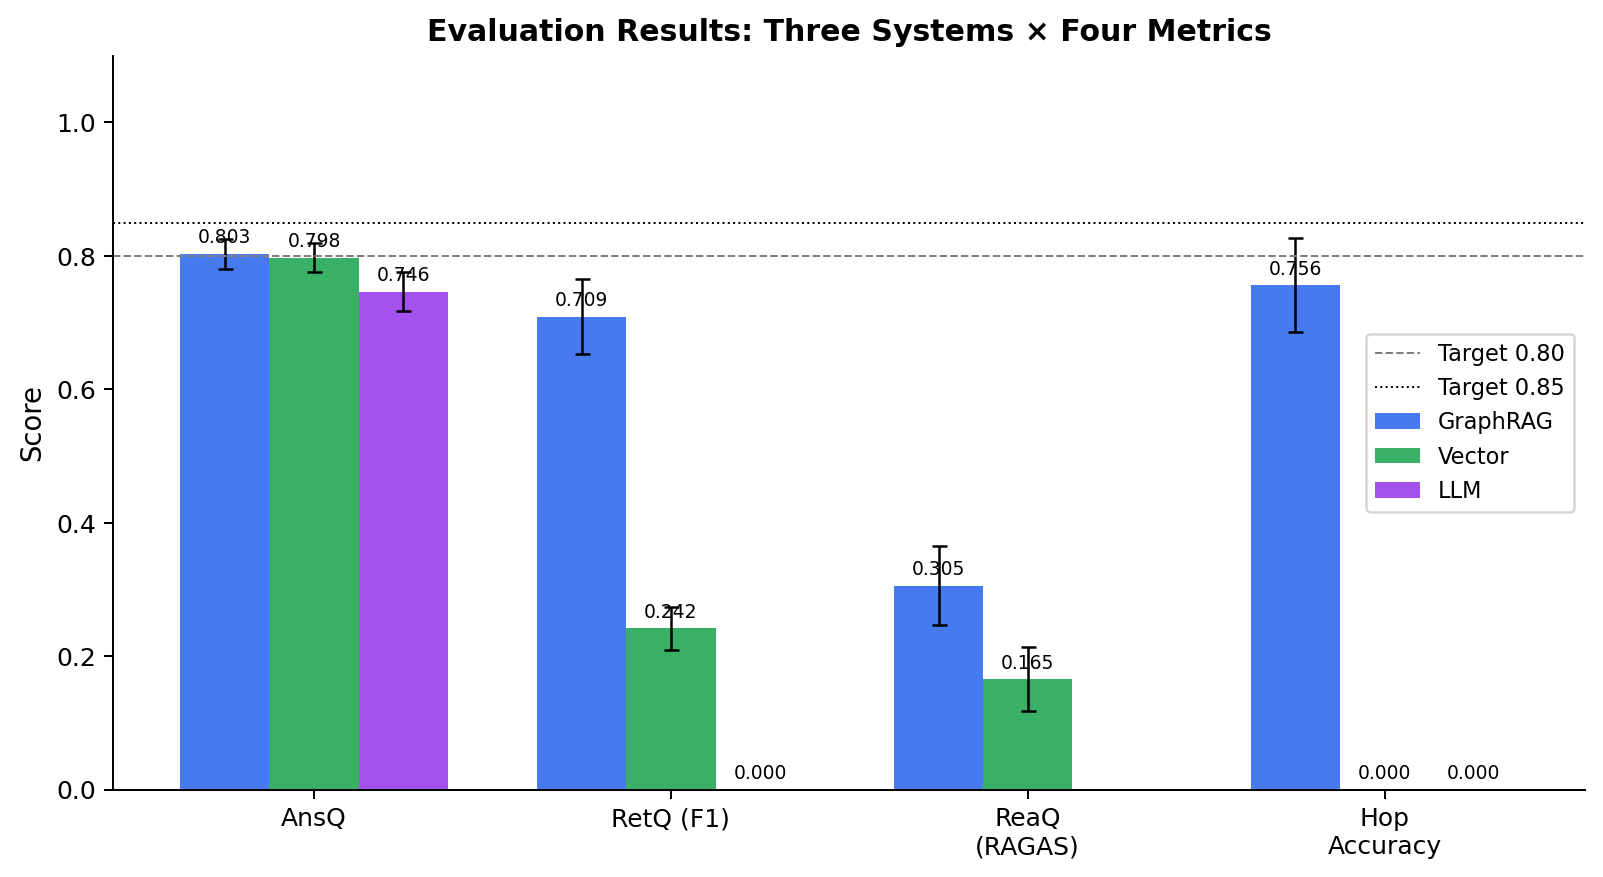
\includegraphics[width=0.88\textwidth]{images/eval_systems_4metrics.png}
    \caption{Perbandingan AnsQ, RetQ F1, \textit{Hop Accuracy}, dan \textit{Faithfulness} tiga sistem.}
    \label{fig:eval_systems_4metrics}
\end{figure}

\renewcommand{\arraystretch}{1.3}
\captionsetup[table]{justification=raggedright,singlelinecheck=false}
\begin{table}[H]
\caption{Perbandingan Skor per Dimensi: Vanilla LLM vs.\ Vector RAG vs.\ Graph RAG}
\label{tbl:baseline_comparison}
\centering
\begin{tabular}{| p{0.28\textwidth} | >{\centering\arraybackslash}p{0.13\textwidth} | >{\centering\arraybackslash}p{0.13\textwidth} | >{\centering\arraybackslash}p{0.13\textwidth} |}
\hline
\textbf{Metrik} & \textbf{Vanilla LLM} ($n{=}102$) & \textbf{Vector RAG} ($n{=}102$) & \textbf{Graph RAG} ($n{=}102$) \\
\hline
\multicolumn{4}{|l|}{\textit{Answer Quality (AnsQ)}} \\
\hline
AnsQ komposit & 0,7469 & 0,7984 & \textbf{0,8031}$^{***\dagger}$ \\
\hline
\quad \textit{Answer Semantic Similarity} & 0,7175 & 0,7503 & 0,7698 \\
\hline
\quad \textit{Syntactic Validity}$^\ddagger$ & 0,8333 & 0,9333 & \textbf{1,0000} \\
\hline
\quad \textit{Schema Compliance}$^\ddagger$ & 0,7931 & \textbf{0,9655} & 0,9259 \\
\hline
\multicolumn{4}{|l|}{\textit{Retrieval Quality (RetQ)}} \\
\hline
RetQ F1 & --- & 0,2437 & \textbf{0,7089}$^{***\P}$ \\
\hline
\quad \textit{Precision} & --- & 0,5047 & \textbf{0,8405} \\
\hline
\quad \textit{Recall} & --- & 0,2294 & \textbf{0,7258} \\
\hline
\multicolumn{4}{|l|}{\textit{Reasoning Quality (ReaQ)}} \\
\hline
\textit{Faithfulness} & N/A & 0,1675 ($n{=}80$) & \textbf{0,3055}$^{***\S}$ ($n{=}95$) \\
\hline
\textit{Hop Accuracy} (all) & N/A & N/A$^*$ & \textbf{0,7562} ($n{=}93$) \\
\hline
\quad \textit{Hop Acc.}\ focused ($\leq$15 \textit{edge}) & --- & --- & \textbf{0,9086} ($n{=}50$) \\
\hline
\quad \textit{Hop Acc.}\ closure ($>$15 \textit{edge}) & --- & --- & 0,5791 ($n{=}43$) \\
\hline
\end{tabular}
\end{table}
{\small\noindent --- = tidak berlaku; *** $p<0{,}001$. $^\dagger$ AnsQ: GraphRAG $>$ Vanilla LLM ($p<0{,}001$); GraphRAG vs.\ Vector RAG tidak signifikan ($p_\text{Holm}=0{,}067$). $^\ddagger$ \textit{Syntactic Validity}: $n{=}28/30/30$; \textit{Schema Compliance}: $n{=}27/29/29$ (\textit{fixture} \texttt{serviceaccount\_pod\_binding} dikecualikan --- RBAC di luar \textit{scope definitions}). $^\S$ \textit{Faithfulness}: GraphRAG vs.\ Vector RAG ($\Delta{+}0{,}127$, $p<0{,}001$); N/A vs.\ Vanilla LLM (tanpa \textit{retrieval}). $^*$ \textit{Hop Accuracy} Vector RAG: tidak berlaku (tanpa traversal graf); dikecualikan dari perbandingan. $^\P$ RetQ: *** merujuk pada GraphRAG vs.\ Vector RAG ($\Delta{+}0{,}465$, $p{<}0{,}001$); Vanilla LLM tidak berlaku (---).}


Gambar~\ref{fig:eval_systems_4metrics} dan Tabel~\ref{tbl:baseline_comparison} menunjukkan pola yang konsisten: ketiga sistem memperoleh skor AnsQ yang relatif setara, sementara perbedaan paling signifikan terdapat pada dimensi \textit{retrieval} dan penalaran (RetQ, ReaQ). Penjelasan per-dimensi diuraikan pada subbab-subbab berikut.

% ─────────────────────────────────────────────────────────────────────
\subsection{\textit{Answer Quality} (AnsQ)}
% ─────────────────────────────────────────────────────────────────────

Pada dimensi AnsQ, ketiga sistem mencapai skor yang sebanding: GraphRAG memperoleh AnsQ 0,8031, Vector RAG 0,7976, dan Vanilla LLM 0,7464. Keunggulan GraphRAG terhadap Vanilla LLM signifikan ($\Delta{+}0{,}056$, $p{<}0{,}001$), sedangkan selisih dengan Vector RAG tidak signifikan secara statistik ($\Delta{+}0{,}005$, $p_{\text{Holm}}{=}0{,}067$, Tabel~\ref{tbl:statistical_test}). Hasil ini mengindikasikan bahwa kualitas teks jawaban ditentukan oleh kemampuan generatif LLM, bukan oleh mekanisme \textit{retrieval}.

Pada sub-metrik \textit{syntactic validity} YAML, GraphRAG memperoleh skor sempurna (1,0000, $n{=}28$) dibanding Vector RAG (0,9333) dan Vanilla LLM (0,8333) --- konsisten dengan lapisan validasi YAML yang ditambahkan pada Fase~3 LangGraph. Pada \textit{schema compliance}, Vector RAG memperoleh skor tertinggi (0,9333) dibanding GraphRAG (0,8929): dua \textit{fixture} HPA pada GraphRAG menghasilkan \texttt{apiVersion: autoscaling/v2beta2} (deprecated sejak Kubernetes v1.26), dan \textit{fixture} \texttt{serviceaccount\_pod\_binding} gagal pada ketiga sistem karena alasan struktural.

\begin{figure}[H]
    \centering
    \captionsetup{justification=centering}
    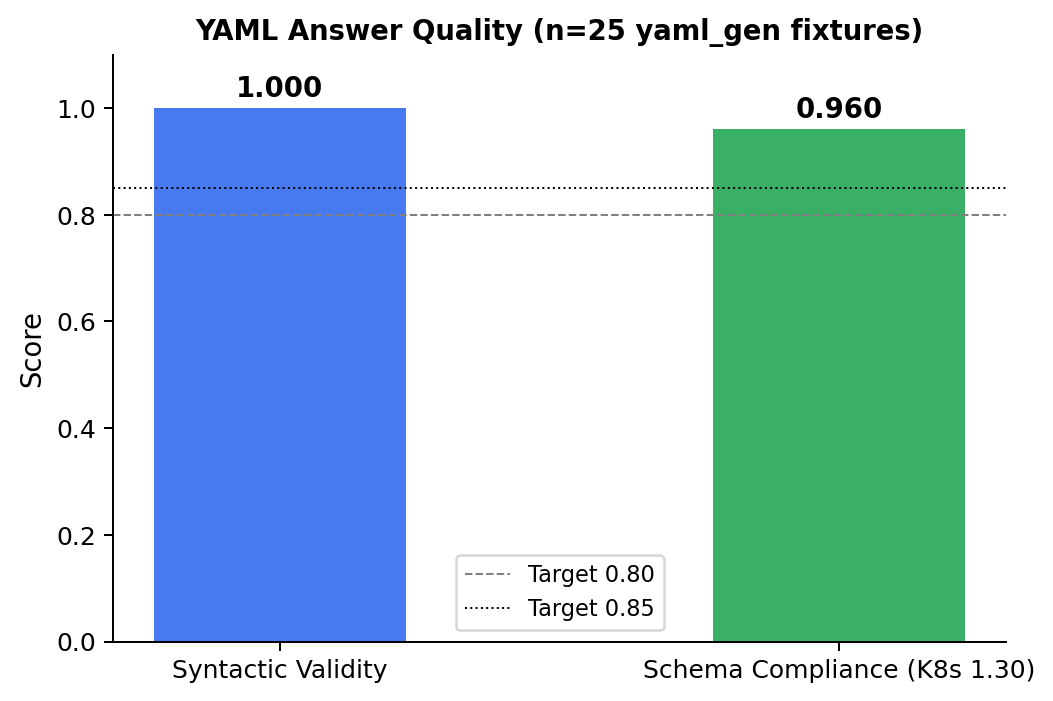
\includegraphics[width=0.82\textwidth]{images/eval_yaml_validity.png}
    \caption{Distribusi \textit{syntactic validity} dan \textit{schema compliance} per sistem pada \textit{fixture} \textit{yaml\_gen}.}
    \label{fig:eval_yaml_validity}
\end{figure}

Tabel~\ref{tbl:ansq_submetrics} merinci skor AnsQ dan sub-metriknya untuk ketiga sistem.

\renewcommand{\arraystretch}{1.3}
\captionsetup[table]{justification=raggedright,singlelinecheck=false}
\begin{table}[H]
\caption{Sub-Metrik \textit{Answer Quality} (AnsQ): Perbandingan Tiga Sistem}
\label{tbl:ansq_submetrics}
\centering
\begin{tabular}{| p{0.32\textwidth} | >{\centering\arraybackslash}p{0.12\textwidth} | >{\centering\arraybackslash}p{0.12\textwidth} | >{\centering\arraybackslash}p{0.12\textwidth} | p{0.16\textwidth} |}
\hline
\textbf{Sub-Metrik} & \textbf{Vanilla LLM} & \textbf{Vector RAG} & \textbf{GraphRAG} & \textbf{Keterangan} \\
\hline
\textit{Answer Semantic Similarity} & 0,7173 & 0,7499 & \textbf{0,7698} & Kemiripan kosinus \textit{embedding} jawaban vs.\ GT \parencite{es_ragas_2023} \\
\hline
\textit{Syntactic Validity} (YAML)$^\dagger$ & 0,8333 ($n{=}30$) & 0,9333 ($n{=}30$) & \textbf{1,0000} ($n{=}28$) & \texttt{yaml.safe\_load} berhasil (v1.30) \\
\hline
\textit{Schema Compliance} (YAML)$^\dagger$ & 0,7667 ($n{=}30$) & \textbf{0,9333} ($n{=}30$) & 0,8929 ($n{=}28$) & Validasi skema Kubernetes v1.30 \\
\hline
\textbf{AnsQ Komposit} & 0,7464 & 0,7976 & \textbf{0,8031} & Rata-rata sub-metrik berlaku \\
\hline
\end{tabular}
\end{table}
{\small\noindent $^\dagger$ Hanya \textit{fixture} \textit{yaml\_gen}. GraphRAG $n{=}28$ vs.\ Vector/LLM $n{=}30$ karena perbedaan \textit{fixture} yang dikerjakan. \textit{Schema Compliance} GraphRAG 0,8929: 2 \textit{fixture} HPA menghasilkan \texttt{apiVersion: autoscaling/v2beta2} (deprecated sejak Kubernetes v1.26); \textit{fixture} \texttt{serviceaccount\_pod\_binding} gagal di ketiga sistem (struktural).}


% ─────────────────────────────────────────────────────────────────────
\subsection{\textit{Retrieval Quality} (RetQ)}
% ─────────────────────────────────────────────────────────────────────

RetQ merupakan dimensi yang paling jelas membedakan ketiga sistem. GraphRAG memperoleh Precision 0,8405 / Recall 0,7258 / F1 0,7089, Vector RAG 0,5018 / 0,2275 / 0,2419, dan Vanilla LLM 0,0000 pada ketiganya. Keunggulan GraphRAG sangat signifikan pada kedua perbandingan ($p{<}0{,}001$, Holm-Bonferroni, Tabel~\ref{tbl:statistical_test}).

Vanilla LLM memperoleh RetQ~0,0000 karena tidak melakukan \textit{retrieval} terstruktur: tidak ada \textit{reasoning path} sehingga tidak ada \textit{node} yang dibandingkan terhadap \textit{ground truth}. Vector RAG mencapai F1~0,2419 melalui \textit{cosine similarity} top-5, namun tanpa traversal \textit{multi-hop}, hanya \textit{seed node} yang terjangkau. GraphRAG dengan \textit{multi-hop traversal} kedalaman adaptif menjangkau \textit{intermediate structural nodes} --- misalnya \textit{DeploymentSpec}, \textit{PodTemplateSpec}, dan \textit{Container} dalam rantai dependensi skema --- menghasilkan Precision yang lebih tinggi sekaligus Recall yang jauh lebih baik dari Vector RAG ($\Delta$Recall $+0{,}498$).

\begin{figure}[H]
    \centering
    \captionsetup{justification=centering}
    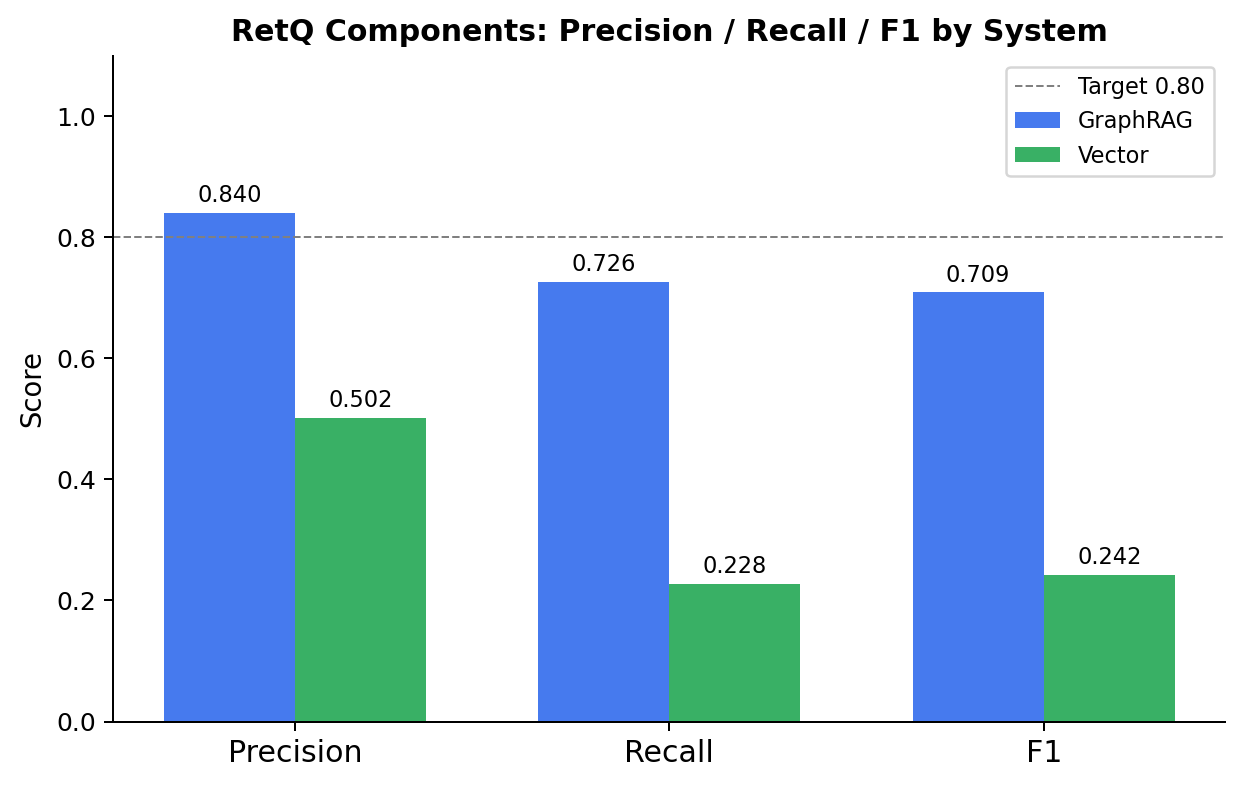
\includegraphics[width=0.88\textwidth]{images/eval_prf_by_system.png}
    \caption{Precision, Recall, dan F1 \textit{retrieval} untuk ketiga sistem.}
    \label{fig:eval_prf_by_system}
\end{figure}

Tabel~\ref{tbl:retq_submetrics} merinci Precision, Recall, dan F1 untuk ketiga sistem.

\renewcommand{\arraystretch}{1.3}
\captionsetup[table]{justification=raggedright,singlelinecheck=false}
\begin{table}[H]
\caption{Sub-Metrik \textit{Retrieval Quality} (RetQ): Perbandingan Tiga Sistem}
\label{tbl:retq_submetrics}
\centering
\begin{tabular}{| p{0.28\textwidth} | >{\centering\arraybackslash}p{0.13\textwidth} | >{\centering\arraybackslash}p{0.13\textwidth} | >{\centering\arraybackslash}p{0.13\textwidth} | p{0.20\textwidth} |}
\hline
\textbf{Sub-Metrik} & \textbf{Vanilla LLM} & \textbf{Vector RAG} & \textbf{Graph RAG} & \textbf{Keterangan} \\
\hline
\textit{Precision} & --- & 0,5047 & \textbf{0,8405} & Fraksi \textit{node} yang di-\textit{retrieve} dan relevan \parencite{manning_ir_2008} \\
\hline
\textit{Recall} & --- & 0,2294 & \textbf{0,7258} & Fraksi \textit{node} relevan yang berhasil di-\textit{retrieve} \\
\hline
\textbf{RetQ F1} & --- & 0,2437 & \textbf{0,7089} & Rata-rata harmonik \textit{Precision} dan \textit{Recall} \\
\hline
\end{tabular}
\end{table}

% ─────────────────────────────────────────────────────────────────────
\subsection{\textit{Reasoning Quality} (ReaQ)}
% ─────────────────────────────────────────────────────────────────────

\textit{Hop accuracy} mengukur \textit{edge recall}: proporsi \textit{edge} dalam \textit{expected path ground truth} yang berhasil dilalui sistem selama traversal \parencite{manning_ir_2008}. GraphRAG memperoleh \textit{hop accuracy} keseluruhan 0,7562 ($n{=}93$ \textit{fixture} dengan \textit{expected\_path} tak kosong).

Analisis stratifikasi berdasarkan ukuran subgraf (Tabel~\ref{tbl:hop_accuracy_stratified}) mengungkapkan pola penting: pada \textit{fixture} \textit{focused} ($\leq$15 \textit{edge}, $n{=}50$), sistem mencapai \textit{hop accuracy} 0,9086 --- hampir seluruh \textit{edge} relevan berhasil dilalui. Sebaliknya, pada \textit{fixture} \textit{closure} ($>$15 \textit{edge}, $n{=}43$), \textit{hop accuracy} turun menjadi 0,5791 karena subgraf besar inheran lebih sulit ditelusuri secara menyeluruh pada kedalaman adaptif.

\renewcommand{\arraystretch}{1.3}
\captionsetup[table]{justification=raggedright,singlelinecheck=false}
\begin{table}[H]
\caption{\textit{Hop Accuracy} GraphRAG Terstratifikasi berdasarkan Ukuran \textit{Ground Truth Path}}
\label{tbl:hop_accuracy_stratified}
\centering
\begin{tabular}{| p{0.38\textwidth} | >{\centering\arraybackslash}p{0.12\textwidth} | >{\centering\arraybackslash}p{0.12\textwidth} | p{0.24\textwidth} |}
\hline
\textbf{Stratum} & \textbf{\textit{n}} & \textbf{\textit{Hop Accuracy}} & \textbf{Deskripsi} \\
\hline
Focused ($\textit{expected\_path} \leq 15$ \textit{edge}) & 50 & \textbf{0,9086} & Subgraf terfokus; sistem berhasil menelusuri hampir seluruh \textit{edge} relevan \\
\hline
Closure ($\textit{expected\_path} > 15$ \textit{edge}) & 43 & 0,5791 & Subgraf besar; pencakupan \textit{edge} lebih sulit secara inheren \\
\hline
\textbf{Keseluruhan} & \textbf{93} & \textbf{0,7562} & \textit{Fixture} dengan \textit{expected\_path} tak kosong \\
\hline
\end{tabular}
\end{table}
{\small\noindent Stratifikasi berdasarkan ukuran \textit{expected\_path} pada \textit{ground truth fixture}. \textit{Hop Accuracy} = \textit{edge recall}: $|E_\text{pred} \cap E_\text{gt}| / |E_\text{gt}|$ \parencite{manning_ir_2008}. \textit{Fixture} dengan \textit{expected\_path} kosong (\textit{conceptual}, sebagian \textit{yaml\_gen}) dikecualikan.}


\textit{Faithfulness} mengukur proporsi klaim dalam jawaban yang dapat dilacak ke \textit{retrieved context} \parencite{es_ragas_2023}. GraphRAG memperoleh \textit{faithfulness} 0,3055 ($n{=}95$), dibandingkan Vector RAG 0,1654 ($n{=}81$). Selisih ini signifikan ($\Delta{+}0{,}127$, $p{<}0{,}001$), menunjukkan bahwa konteks berbasis graf meningkatkan proporsi klaim yang terdukung.

\begin{figure}[H]
    \centering
    \captionsetup{justification=centering}
    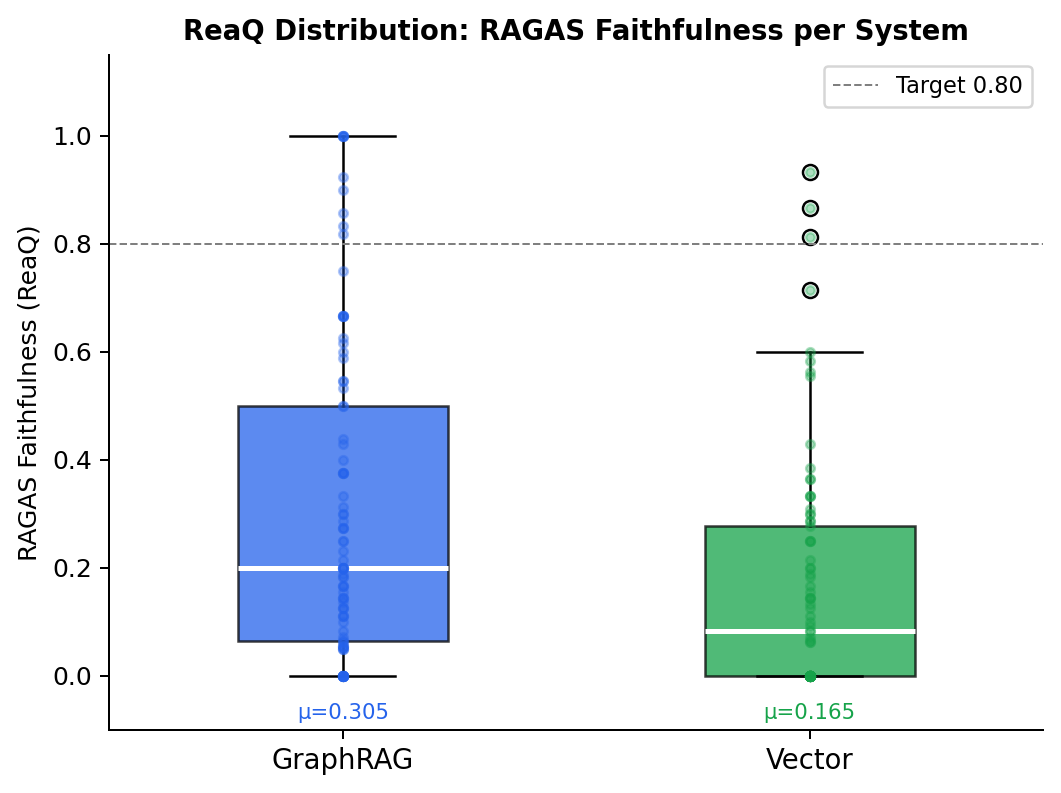
\includegraphics[width=0.82\textwidth]{images/eval_ragas_faithfulness_dist.png}
    \caption{Distribusi skor \textit{faithfulness} GraphRAG vs.\ Vector RAG.}
    \label{fig:eval_ragas_faithfulness_dist}
\end{figure}

Nilai 0,3055 tetap lebih rendah dari ambang 0,80; komposisi dan interpretasi hasil ini dianalisis mendalam pada Subbab~\ref{subsec:analisis-reaq}.

\renewcommand{\arraystretch}{1.3}
\captionsetup[table]{justification=raggedright,singlelinecheck=false}
\begin{table}[H]
\caption{Perbandingan \textit{Faithfulness}: GraphRAG vs.\ Vector RAG}
\label{tbl:faithfulness_comparison}
\centering
\begin{tabular}{| p{0.30\textwidth} | >{\centering\arraybackslash}p{0.14\textwidth} | >{\centering\arraybackslash}p{0.14\textwidth} | >{\centering\arraybackslash}p{0.10\textwidth} | >{\centering\arraybackslash}p{0.14\textwidth} |}
\hline
\textbf{Metrik} & \textbf{Vector RAG} & \textbf{Graph RAG} & \textbf{$\Delta$} & \textbf{Sig} \\
\hline
\textit{Faithfulness} & 0,1675 & \textbf{0,3055} & $+0{,}127$ & $p<0{,}001$ *** \\
\hline
\end{tabular}
\end{table}
{\small\noindent Uji Wilcoxon + \textit{paired bootstrap} 1.000 iterasi, $H_1$: GraphRAG $>$ Vector RAG. \textit{Faithfulness} = proporsi klaim dalam jawaban yang dapat dilacak ke \textit{retrieved context} \parencite{es_ragas_2023}. N/A untuk Vanilla LLM (tidak ada \textit{retrieval context}). \textit{Catatan}: nilai absolut mencerminkan desain \textit{open-book} sistem --- 55,6\% klaim bersumber dari pengetahuan parametrik LLM.}


Tabel~\ref{tbl:reaq_submetrics} merangkum seluruh sub-metrik ReaQ.

\renewcommand{\arraystretch}{1.3}
\captionsetup[table]{justification=raggedright,singlelinecheck=false}
\begin{table}[H]
\caption{Sub-Metrik \textit{Reasoning Quality} (ReaQ) Sistem GraphRAG}
\label{tbl:reaq_submetrics}
\centering
\begin{tabular}{| p{0.38\textwidth} | c | p{0.36\textwidth} |}
\hline
\textbf{Sub-Metrik} & \textbf{Nilai} & \textbf{Keterangan} \\
\hline
\textit{Hop-Accuracy (edge recall)} & 0,7562 ($n{=}93$) & Fraksi \textit{edge} GT yang dilalui traversal \parencite{manning_ir_2008} \\
\hline
\quad Focused ($\leq$15 \textit{edge}) & \textbf{0,9086} ($n{=}50$) & Subgraf terfokus: pencakupan tinggi \\
\hline
\quad Closure ($>$15 \textit{edge}) & 0,5791 ($n{=}43$) & Subgraf besar: pencakupan lebih terbatas \\
\hline
\textit{Faithfulness} & 0,3055 ($n{=}95$) & Proporsi klaim jawaban yang terdukung \textit{context} \parencite{es_ragas_2023} \\
\hline
\end{tabular}
\end{table}
{\small\noindent \textit{Hop-Accuracy (edge recall)} N/A untuk \textit{fixture} dengan \textit{expected\_path} kosong (dirata-rata dari $n{=}93$). \textit{Faithfulness} rendah (0,3055) mencerminkan desain \textit{open-book}: 55,6\% klaim parametrik (dekomposisi $n{=}102$); bukan defek sistem. ReaQ Vanilla LLM: N/A (tidak ada \textit{retrieval context} untuk dievaluasi).}


% ─────────────────────────────────────────────────────────────────────
\subsection{Analisis Per-Kategori}
\label{subsec:domain-metrics}
% ─────────────────────────────────────────────────────────────────────

Tabel~\ref{tbl:category_scores} menyajikan skor per kategori \textit{fixture} untuk sistem GraphRAG.

\begin{figure}[H]
    \centering
    \captionsetup{justification=centering}
    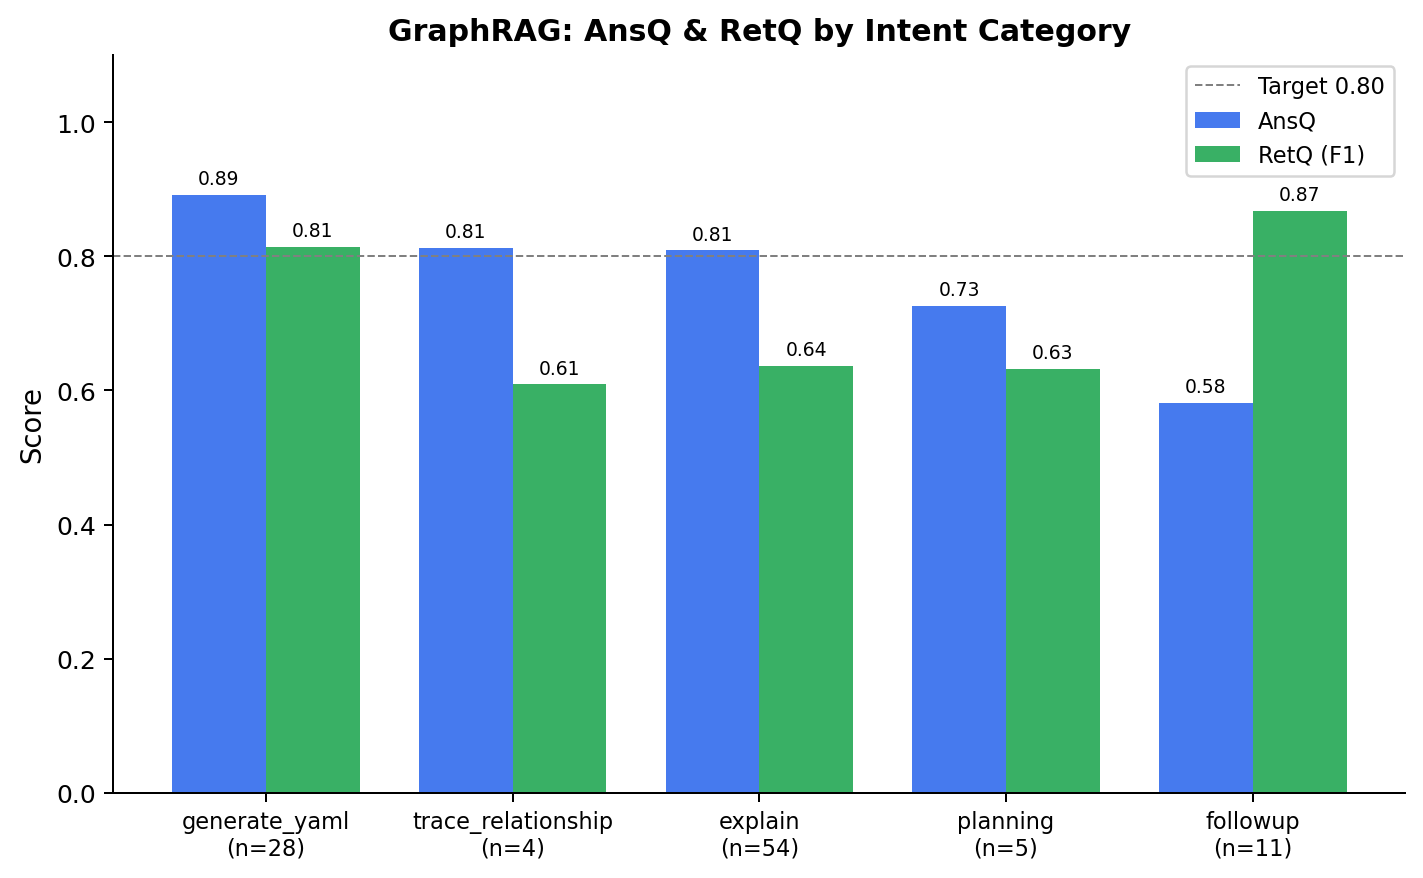
\includegraphics[width=0.90\textwidth]{images/eval_by_intent.png}
    \caption{AnsQ, RetQ F1, dan \textit{Hop Accuracy} GraphRAG per kategori \textit{fixture}.}
    \label{fig:eval_by_intent}
\end{figure}

\renewcommand{\arraystretch}{1.3}
\captionsetup[table]{justification=raggedright,singlelinecheck=false}
\begin{table}[H]
\caption{Skor Evaluasi Sistem GraphRAG per Kategori \textit{Fixture} ($n{=}102$)}
\label{tbl:category_scores}
\centering
\begin{tabular}{| p{0.20\textwidth} | c | c | c | c |}
\hline
\textbf{Kategori} & \textbf{\textit{n}} & \textbf{AnsQ} & \textbf{RetQ} & \textbf{ReaQ} \\
\hline
\textit{yaml\_gen}       & 25 & \textbf{0,910} & \textbf{0,817} & 0,567 \\
\hline
\textit{followup}        & 12 & 0,590 & 0,826 & 0,491 \\
\hline
\textit{command}         &  3 & 0,803 & 0,781 & 0,449 \\
\hline
\textit{relationship}    & 18 & 0,812 & 0,590 & 0,439 \\
\hline
\textit{conceptual}      & 25 & 0,818 & 0,708 & 0,629 \\
\hline
\textit{planning}        &  5 & 0,726 & 0,632 & \textbf{0,746} \\
\hline
\textit{troubleshooting} &  5 & 0,867 & 0,534 & 0,336 \\
\hline
\textit{realworld}       &  9 & 0,739 & 0,611 & 0,386 \\
\hline
\textbf{Keseluruhan}     & \textbf{102} & \textbf{0,803} & \textbf{0,709} & \textbf{0,531} \\
\hline
\end{tabular}
\end{table}

Sistem GraphRAG memperoleh RetQ tertinggi pada \textit{yaml\_gen} (0,817) dan \textit{followup} (0,826), mencerminkan efektivitas traversal bertingkat pada kueri yang secara inheren membutuhkan konteks relasional antar-\textit{resource}. \textit{Hop accuracy} tertinggi diraih oleh kategori \textit{followup} (0,933) dan \textit{planning} (1,000) yang memang membutuhkan traversal multi-\textit{hop}. Kategori \textit{relationship} memperoleh \textit{faithfulness} tertinggi (0,389) karena jawaban yang menyatakan ulang relasi struktural dapat dilacak langsung ke konteks graf. Sebaliknya, \textit{yaml\_gen} memperoleh \textit{faithfulness} terendah (0,206): sistem mengisi nilai YAML konkret dari konvensi praktik, bukan dari deskripsi skema, sehingga \textit{faithfulness} secara konstruk tidak sepenuhnya \textit{applicable} untuk pembangkitan kode. Pola ini berkontribusi pada kasus paradoks (\textit{faith}~$\leq$~0,30 tetapi AnsQ~$\geq$~0,70) yang dianalisis lebih lanjut pada Subbab~\ref{subsec:analisis-reaq}.

% ─────────────────────────────────────────────────────────────────────
\section{Analisis Evaluasi}
\label{sec:analisis-evaluasi}
% ─────────────────────────────────────────────────────────────────────

Bagian ini menganalisis hasil pada Bagian~\ref{sec:hasil-evaluasi} dari enam sudut: per-dimensi (AnsQ, RetQ, ReaQ), studi mekanisme internal (kedalaman traversal, ablasi, kondisi batas), perbandingan statistik tiga sistem, dan sintesis lintas-metrik.

% ─────────────────────────────────────────────────────────────────────
\subsection{Analisis \textit{Answer Quality} (AnsQ)}
\label{subsec:analisis-ansq}
% ─────────────────────────────────────────────────────────────────────

Ketiga sistem mencapai AnsQ yang sebanding (GraphRAG 0,803 / Vector RAG 0,798 / Vanilla LLM 0,746), dengan selisih GraphRAG terhadap Vector RAG yang tidak signifikan secara statistik ($\Delta{+}0{,}005$, $p_{\text{Holm}}{=}0{,}067$). Pola ini mencerminkan karakteristik \textit{LLM-bound}: kualitas teks jawaban ditentukan oleh kapabilitas generatif model bahasa, bukan oleh mekanisme \textit{retrieval}. Selama model yang digunakan sama (GPT-4o-mini), perbedaan AnsQ antarsistem akan selalu kecil. Implikasinya, AnsQ bukan pembeda utama antara arsitektur GraphRAG dan Vector RAG; keunggulan komparatif terukur terletak pada RetQ dan ReaQ.

% ─────────────────────────────────────────────────────────────────────
\subsection{Analisis \textit{Retrieval Quality} (RetQ)}
\label{subsec:analisis-retq}
% ─────────────────────────────────────────────────────────────────────

RetQ merupakan dimensi paling diskriminatif: GraphRAG mengungguli Vector RAG sebesar $+0{,}465$ F1 ($p{<}0{,}001$) dan Vanilla LLM sebesar $+0{,}709$ ($p{<}0{,}001$). Keunggulan ini bersumber dari traversal \textit{multi-hop} yang menjangkau \textit{intermediate structural nodes} --- misalnya rantai \textit{Deployment}~$\to$~\textit{DeploymentSpec}~$\to$~\textit{PodTemplateSpec}~$\to$~\textit{Container} --- yang tidak dapat dicapai oleh \textit{cosine similarity} top-5 Vector RAG. Analisis lebih lanjut tentang komponen pendorong RetQ disajikan pada Subbab~\ref{subsec:studi-mekanisme}: ablasi A2 (\textit{no\_multihop}) menghilangkan $-0{,}656$ pp RetQ, dan T1 (18-\textit{edge} semantik) berkontribusi $+0{,}152$ pp.

% ─────────────────────────────────────────────────────────────────────
\subsection{Analisis \textit{Reasoning Quality} (ReaQ)}
\label{subsec:analisis-reaq}
% ─────────────────────────────────────────────────────────────────────

\textit{Hop accuracy} keseluruhan 0,756 mencerminkan \textit{trade-off} traversal yang bersifat inheran. Pada \textit{fixture} \textit{focused} ($\leq$15 \textit{edge}, $n{=}50$), sistem mencapai 0,909 --- hampir seluruh relasi relevan berhasil dilalui. Skor turun ke 0,579 pada \textit{fixture} \textit{closure} ($>$15 \textit{edge}, $n{=}43$) karena kedalaman adaptif $d{=}2$ tidak dapat menelusuri semua cabang subgraf besar secara menyeluruh. Pola ini terdokumentasi pada eksperimen kedalaman (Subbab~\ref{subsec:studi-mekanisme}): menambah kedalaman meningkatkan \textit{hop accuracy} (lihat $d{=}4$, 0,901) namun menurunkan presisi RetQ, sehingga $d{=}2$ tetap optimal secara agregat.

\textit{Faithfulness} 0,3055 berada jauh di bawah ambang 0,80, namun interpretasi angka ini memerlukan pemahaman desain sistem. \texttt{prompts.py} Aturan~1 secara eksplisit menyatakan \textit{``If Retrieved Data is empty or does not cover the specific concept asked, answer using your general Kubernetes knowledge''}. Sistem ini memang dirancang \textit{open-book}: \textit{knowledge graph} berfungsi sebagai \textit{scaffold} struktural, dan LLM diizinkan melengkapi jawaban dengan pengetahuan parametrik ketika informasi tidak tersedia dalam konteks yang di-\textit{retrieve}.

Untuk mengkuantifikasi seberapa besar porsi jawaban bersumber dari graf versus ingatan LLM, seluruh 102 \textit{fixture} dianalisis menggunakan dekomposisi klaim berbasis GPT-4o: tiap klaim diklasifikasikan sebagai \textit{supported} (terdukung konteks), \textit{modality} (isi didukung, beda formulasi deklaratif~$\to$~prosedural), \textit{partial}, atau \textit{absent} (tidak ada di konteks). Hasilnya disajikan pada Tabel~\ref{tbl:faith_decomposition}.

\renewcommand{\arraystretch}{1.3}
\captionsetup[table]{justification=raggedright,singlelinecheck=false}
\begin{table}[H]
\caption{Dekomposisi Klaim Jawaban GraphRAG: Sumber Pengetahuan DOCUMENT vs.\ PARAMETRIC}
\label{tbl:faith_decomposition}
\centering
\begin{tabular}{| >{\raggedright\arraybackslash}p{0.18\textwidth} | >{\centering\arraybackslash}p{0.18\textwidth} | >{\centering\arraybackslash}p{0.13\textwidth} | >{\centering\arraybackslash}p{0.09\textwidth} | >{\raggedright\arraybackslash}p{0.25\textwidth} |}
\hline
\textbf{Kategori} & \textbf{Sumber} & \textbf{Jumlah Klaim} & \textbf{\%} & \textbf{Keterangan} \\
\hline
\textit{supported} & DOCUMENT & 258 & 31,5 & Klaim terlacak ke konteks graf \\
\hline
\textit{modality} & DOCUMENT & 81 & 9,9 & Isi didukung, beda formulasi deklaratif~$\to$~prosedural \\
\hline
\textit{partial} & (abu-abu) & 24 & 2,9 & Sebagian terdukung konteks \\
\hline
\textit{absent} & PARAMETRIC & 455 & 55,6 & Klaim dari ingatan parametrik LLM \\
\hline
\hline
\textbf{Total DOCUMENT} & & \textbf{339} & \textbf{41,4} & \textit{supported} $+$ \textit{modality} \\
\hline
\textbf{Total PARAMETRIC} & & \textbf{455} & \textbf{55,6} & \textit{absent} \\
\hline
\end{tabular}
\end{table}


Dari 818 klaim, \textbf{55,6\% bersumber dari pengetahuan parametrik} (\textit{absent}) --- dan hanya 41,4\% dapat dilacak ke konteks graf secara jelas (\textit{supported}~$+$~\textit{modality}). Pola ini konsisten pada kedua subset: 55,6\% parametrik untuk \textit{fixture} berbasis skema ($n{=}86$) maupun 55,8\% untuk \textit{fixture} \textit{free-text} ($n{=}16$), mengindikasikan bahwa desain \textit{open-book} berdampak sistemik, bukan artefak satu kelompok pertanyaan saja.

Pertanyaan yang muncul kemudian adalah: mengapa \textit{faithfulness} rendah (0,306) tetapi AnsQ tetap tinggi (0,803)? Gambar~\ref{fig:faith_vs_ansq_scatter} memvisualisasikan sebaran pasangan skor keduanya per \textit{fixture}.

\begin{figure}[H]
    \centering
    \captionsetup{justification=centering}
    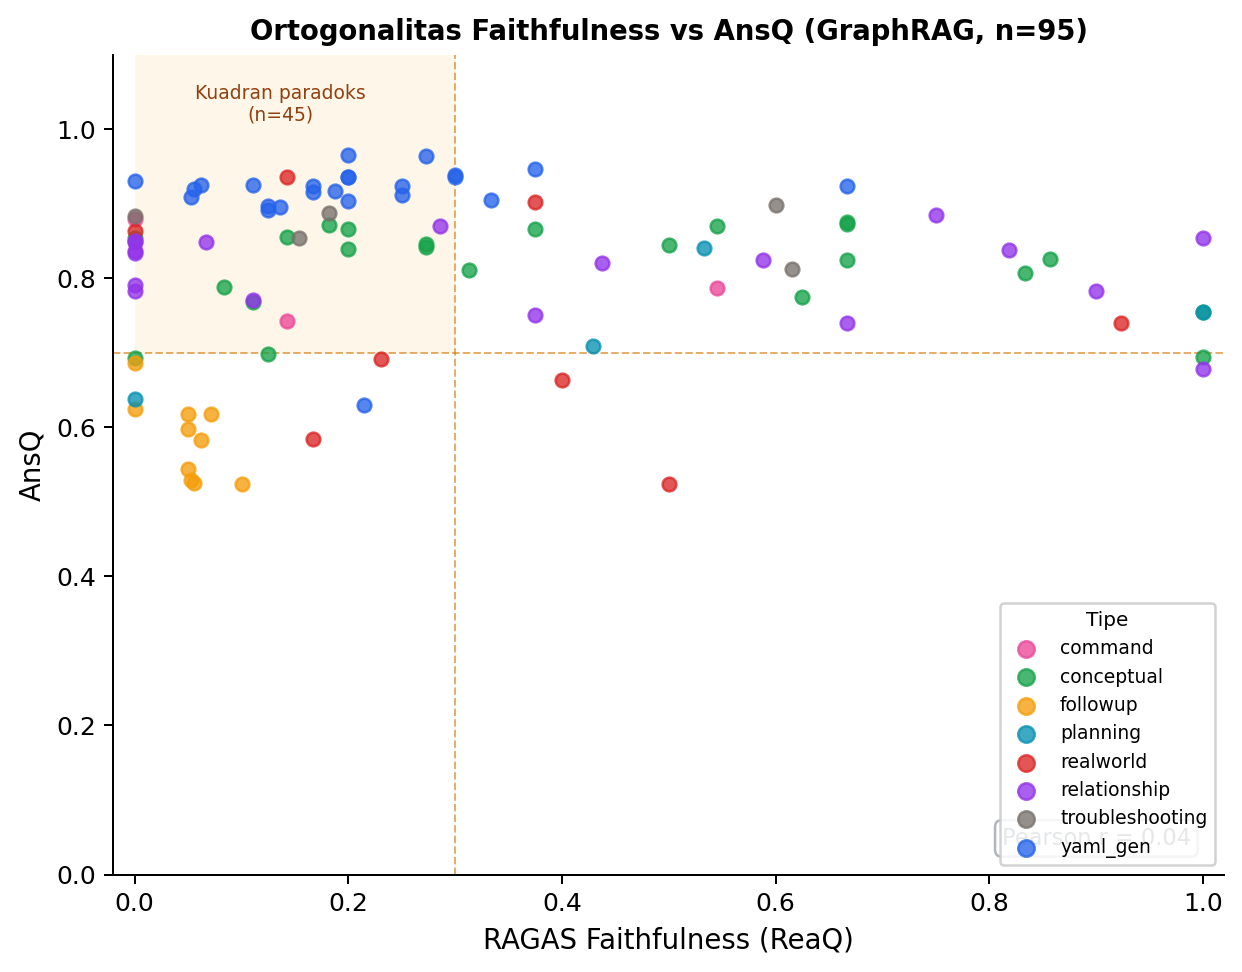
\includegraphics[width=0.82\textwidth]{images/eval_faith_vs_ansq_scatter.png}
    \caption{Sebaran \textit{faithfulness} vs.\ AnsQ per \textit{fixture} GraphRAG ($n{=}95$ pasangan valid). Kuadran paradoks (kiri atas, \textit{faith}~$\leq$~0,30, AnsQ~$\geq$~0,70) diarsir. Pearson $r{=}0{,}23$.}
    \label{fig:faith_vs_ansq_scatter}
\end{figure}

Korelasi Pearson $r{=}0{,}23$ (hampir nol) membuktikan bahwa \textit{faithfulness} dan AnsQ \textbf{ortogonal}: tinggi-rendahnya \textit{faithfulness} tidak memprediksi kualitas jawaban. Dari 102 \textit{fixture}, \textbf{41 masuk kuadran paradoks} (\textit{faith}~$\leq$~0,30 tetapi AnsQ~$\geq$~0,70), didominasi tipe \textit{yaml\_gen} (\textit{faith} rata-rata 0,206, AnsQ 0,910): LLM mengisi nilai YAML konkret dari ingatan parametrik, menghasilkan jawaban yang tepat secara teknis namun tidak terlacak ke konteks graf --- perilaku yang memang dikehendaki desain \textit{open-book}.

Variasi antarkategori memperkuat temuan ini. Satu-satunya kategori dengan \textit{faithfulness} DAN AnsQ sama-sama rendah adalah \textit{followup} (\textit{faith} 0,044, AnsQ 0,590), yang mencerminkan limitasi genuine sistem pada kueri multi-\textit{turn} tanpa retensi konteks antarsesi. Sebaliknya, kategori \textit{relationship} memperoleh \textit{faithfulness} tertinggi (0,389) karena menyatakan ulang relasi struktural yang dapat dilacak langsung ke konteks graf. Terakhir, perlu dibedakan dua analisis ini: \textit{Faithfulness} 0,3055 dihitung oleh judge GPT-4o-mini pada $n{=}95$ \textit{fixture} dan merupakan metrik resmi yang dibandingkan antarsistem; sedangkan dekomposisi klaim pada Tabel~\ref{tbl:faith_decomposition} menggunakan judge GPT-4o pada $n{=}102$ \textit{fixture} untuk mengidentifikasi sumber klaim (DOCUMENT vs.\ PARAMETRIC) --- ini analisis diagnostik yang meng-\textit{corroborate} metrik resmi, bukan nilai \textit{faithfulness} kedua.

% ─────────────────────────────────────────────────────────────────────
\subsection{Studi Mekanisme}
\label{subsec:studi-mekanisme}
% ─────────────────────────────────────────────────────────────────────

Tiga eksperimen berikut menganalisis mekanisme internal GraphRAG secara terukur, memperinci faktor pendorong RetQ dan ReaQ yang telah diidentifikasi pada subbab-subbab sebelumnya.

% ─────────────────────────────────────────────────────────────────────
\subsection{Sensitivitas Kedalaman Traversal}
% ─────────────────────────────────────────────────────────────────────

Eksperimen kedalaman mengeksplorasi pengaruh kedalaman traversal $d$ terhadap tiga dimensi evaluasi. Tabel~\ref{tbl:depth_sensitivity} menyajikan hasil untuk empat nilai $d$ yang diuji.

\renewcommand{\arraystretch}{1.3}
\captionsetup[table]{justification=raggedright,singlelinecheck=false}
\begin{table}[H]
\caption{Sensitivitas Kedalaman Traversal: Skor per Dimensi ($n{=}102$)}
\label{tbl:depth_sensitivity}
\centering
\begin{tabular}{| c | c | c | c | p{0.30\textwidth} |}
\hline
\textbf{Kedalaman ($d$)} & \textbf{RetQ F1} & \textbf{AnsQ} & \textbf{\textit{Hop Accuracy}} & \textbf{Catatan} \\
\hline
$d=1$ & 0,3666 & 0,7815 & 0,2574 & \textit{Retrieval} dangkal; banyak relasi tidak terjangkau \\
\hline
$d=2$ (\textit{default}) & \textbf{0,7089} & \textbf{0,8031} & 0,7562 & Titik optimum RetQ dan AnsQ \\
\hline
$d=3$ & 0,6593 & 0,7891 & \textbf{0,9007} & HopAcc tertinggi; RetQ mulai turun \\
\hline
$d=4$ & 0,6113 & 0,7828 & 0,9007 & RetQ turun lebih lanjut; presisi berkurang \\
\hline
$d=5$ & 0,5838 & 0,7817 & 0,8760 & HopAcc menurun dari $d=3$--$d=4$; \textit{noise} meningkat \\
\hline
\end{tabular}
\end{table}


\begin{figure}[H]
    \centering
    \captionsetup{justification=centering}
    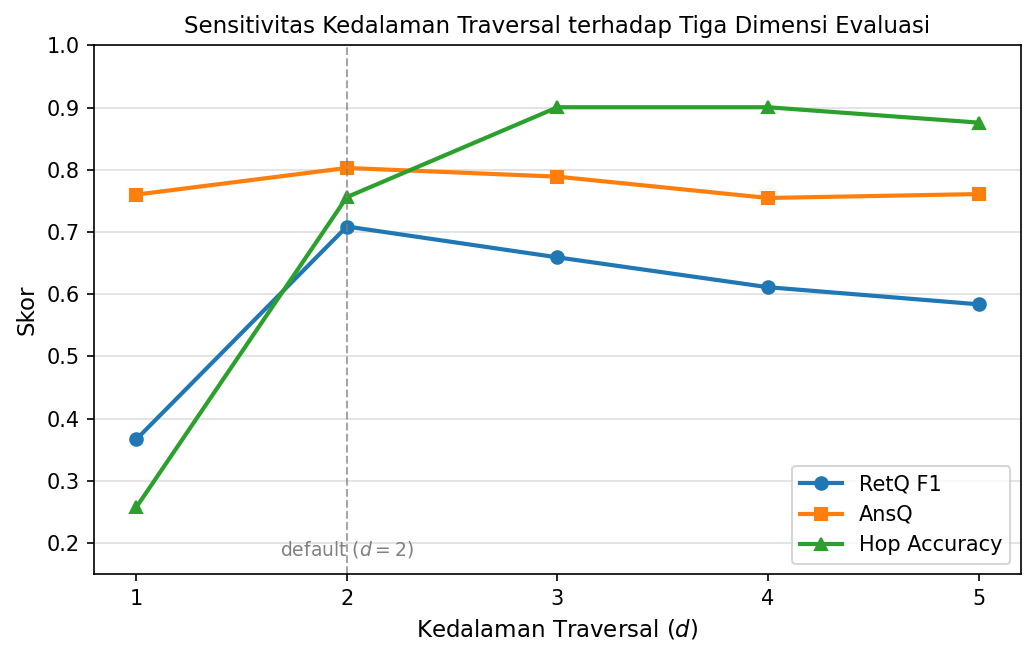
\includegraphics[width=0.88\textwidth]{images/depth_sensitivity_aggregate.png}
    \caption{Sensitivitas RetQ F1, AnsQ, dan \textit{Hop Accuracy} terhadap kedalaman traversal $d$.}
    \label{fig:depth_sensitivity_bab6}
\end{figure}

Kedalaman $d{=}2$ merupakan titik optimal untuk RetQ F1 (0,7089) dan AnsQ (0,8031). Pada $d{=}1$, RetQ turun drastis menjadi 0,3666 karena \textit{retrieval} dangkal hanya menjangkau \textit{seed node} tanpa konteks dependensi skema. Pada $d{=}4$ dan $d{=}5$, \textit{Hop Accuracy} naik (0,9007 dan 0,8760) --- sistem menelusuri lebih banyak \textit{edge} relevan --- tetapi RetQ justru turun (0,6113 dan 0,5838) karena traversal lebih dalam menarik \textit{node} tambahan yang menurunkan presisi. Pola ini mengkonfirmasi \textit{trade-off} antara \textit{edge recall} dan presisi \textit{retrieval}: kedalaman adaptif $d{=}2$ (default) mempertahankan keseimbangan terbaik untuk mayoritas kueri.

% ─────────────────────────────────────────────────────────────────────
\subsection{Analisis Internal: \textit{Ablation Study}}
\label{sec:ablation-study}
% ─────────────────────────────────────────────────────────────────────

\textit{Ablation study} dilakukan untuk memverifikasi kontribusi terukur tiap komponen sistem GraphRAG. Tujuh konfigurasi ablasi (A1--A7) dirancang sehingga tiap konfigurasi menonaktifkan tepat satu komponen, dievaluasi terhadap 103 \textit{fixture}. Tabel~\ref{tbl:ablation_results} menyajikan skor absolut dan selisih terhadap \textit{baseline} (18-\textit{edge}), sedangkan Tabel~\ref{tbl:ablation_significance} menyajikan signifikansi statistiknya.

\begin{figure}[H]
    \centering
    \captionsetup{justification=centering}
    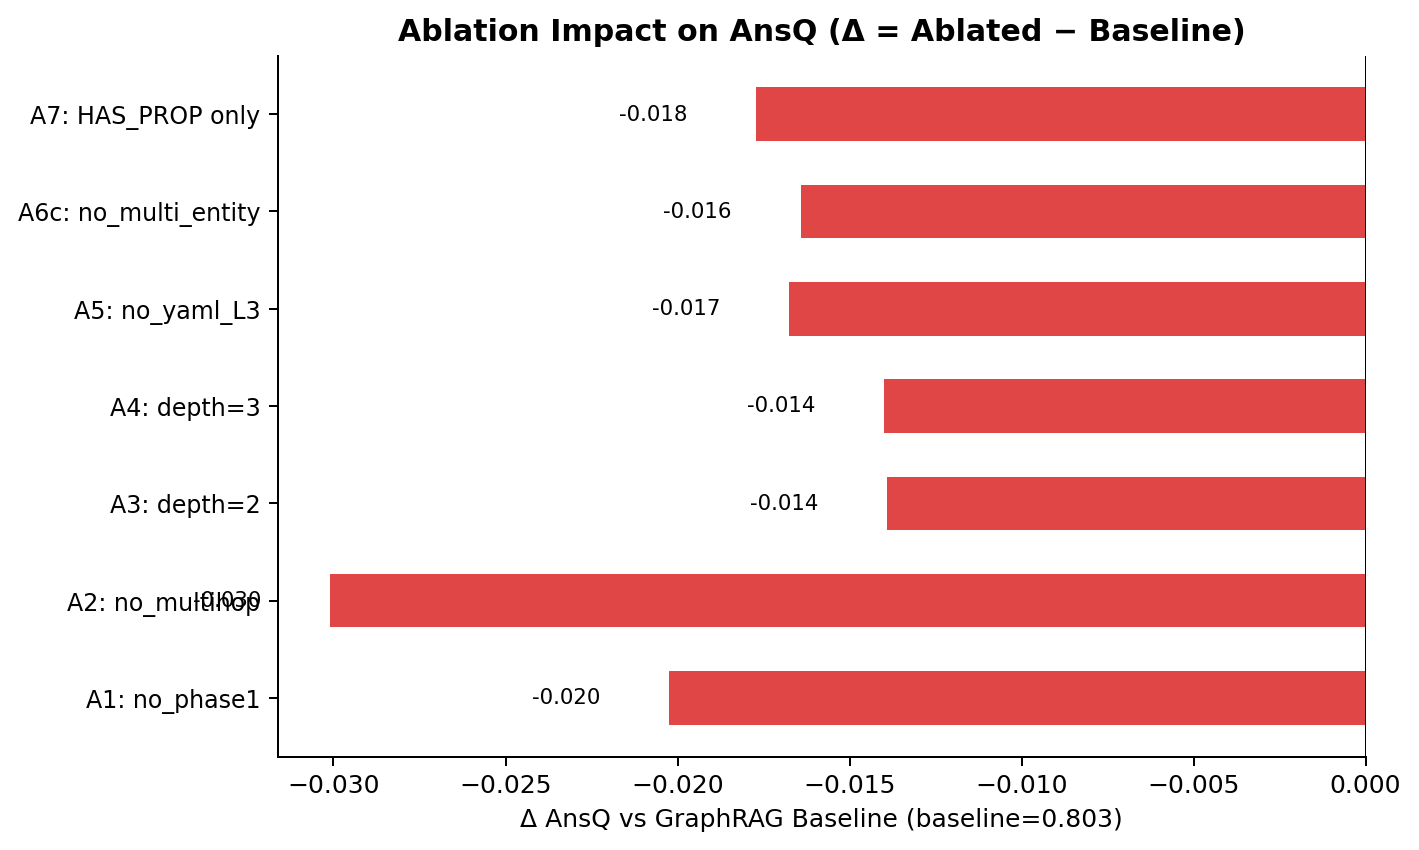
\includegraphics[width=0.90\textwidth]{images/eval_ablation_impact.png}
    \caption{Penurunan RetQ F1 dan \textit{Hop Accuracy} pada tiap konfigurasi ablasi.}
    \label{fig:eval_ablation_impact}
\end{figure}

\renewcommand{\arraystretch}{1.3}
\captionsetup[table]{justification=raggedright,singlelinecheck=false}
\begin{table}[H]
\caption{\textit{Ablation Study}: Skor Absolut dan Selisih terhadap \textit{Baseline} GraphRAG ($n{=}102$)}
\label{tbl:ablation_results}
\centering
\begin{footnotesize}
\setlength{\tabcolsep}{5pt}
\begin{tabular}{| p{0.24\textwidth} | r | r | r | r | r | r |}
\hline
\textbf{Konfigurasi} & \textbf{AnsQ} & \textbf{$\Delta$AnsQ} & \textbf{RetQ F1} & \textbf{$\Delta$RetQ} & \textbf{HopAcc} & \textbf{$\Delta$HopAcc} \\
\hline
\textbf{Baseline (18 \textit{edge})} & $0{,}8031$ & --- & $0{,}7089$ & --- & $0{,}7562$ & --- \\
\hline
A1 \textit{no\_phase1}       & $0{,}7829$ & $-0{,}0202$ & $0{,}4001$ & $-0{,}3088$ & $0{,}4164$ & $-0{,}3398$ \\
\hline
A2 \textit{no\_multihop}     & $0{,}7730$ & $-0{,}0301$ & $0{,}0527$ & $-0{,}6562$ & $0{,}0560$ & $-0{,}7002$ \\
\hline
A3 \textit{depth=2 fixed}    & $0{,}7892$ & $-0{,}0139$ & $0{,}5857$ & $-0{,}1232$ & $0{,}6090$ & $-0{,}1472$ \\
\hline
A4 \textit{depth=3 fixed}    & $0{,}7891$ & $-0{,}0140$ & $0{,}6593$ & $-0{,}0496$ & $0{,}9007$ & $+0{,}1445$ \\
\hline
A5 \textit{no\_yaml\_layer3} & $0{,}7864$ & $-0{,}0167$ & $0{,}6524$ & $-0{,}0565$ & $0{,}7599$ & $-0{,}0037$ \\
\hline
A6 \textit{no\_multi\_ent.} & $0{,}7867$ & $-0{,}0164$ & $0{,}6979$ & $-0{,}0110$ & $0{,}7493$ & $-0{,}0069$ \\
\hline
A7 \textit{HAS\_PROP only}   & $0{,}7854$ & $-0{,}0177$ & $0{,}5573$ & $-0{,}1516$ & $0{,}5242$ & $-0{,}2320$ \\
\hline
\end{tabular}
\end{footnotesize}
\end{table}
{\footnotesize\noindent $\Delta$ = Baseline $-$ Ablasi; nilai positif = komponen berkontribusi positif.}


\renewcommand{\arraystretch}{1.3}
\captionsetup[table]{justification=raggedright,singlelinecheck=false}
\begin{table}[H]
\caption{Signifikansi Statistik \textit{Ablation Study} per Faktor (Wilcoxon + \textit{Bootstrap}, $p$-\textit{value})}
\label{tbl:ablation_significance}
\centering
\begin{footnotesize}
\setlength{\tabcolsep}{5pt}
\begin{tabular}{| p{0.22\textwidth} | c | c | c | c | c | c |}
\hline
\textbf{Ablasi} & \textbf{AnsQ} & \textbf{RetQ} & \textbf{ReaQ} & \textbf{PCov} & \textbf{HopAcc} & \textbf{RGA} \\
\hline
A1 \textit{no\_phase1}       & $0{,}591$ & $<0{,}001$ & $<0{,}001$ & $<0{,}001$ & $<0{,}001$ & $<0{,}001$ \\
\hline
A2 \textit{no\_multihop}     & $0{,}060$ & $<0{,}001$ & $<0{,}001$ & $<0{,}001$ & $<0{,}001$ & $<0{,}001$ \\
\hline
A3 \textit{depth=2 fixed}    & $0{,}242$ & $<0{,}001$ & $<0{,}001$ & $0{,}010$  & $<0{,}001$ & $0{,}128$  \\
\hline
A4 \textit{depth=3 fixed}    & $0{,}774$ & $0{,}493$  & $0{,}104$  & $0{,}997$  & $0{,}126$  & $0{,}673$  \\
\hline
A5 \textit{no\_yaml\_layer3} & $0{,}133$ & $0{,}250$  & $0{,}007$  & $0{,}841$  & $0{,}079$  & $0{,}090$  \\
\hline
A6c \textit{no\_multi\_ent.} & $0{,}527$ & $0{,}219$  & $0{,}727$  & $0{,}015$  & $0{,}977$  & $0{,}017$  \\
\hline
\multicolumn{7}{l}{\scriptsize PCov = \textit{Path Coverage}; HopAcc = \textit{Hop Accuracy}.} \\
\multicolumn{7}{l}{\scriptsize $H_1$: \textit{baseline} lebih tinggi dari varian ablasi. Nilai $< 0{,}05$ mengindikasikan komponen berkontribusi.} \\
\end{tabular}
\end{footnotesize}
\end{table}


\textbf{A2 (\textit{no\_multihop})} menghasilkan penurunan terbesar: RetQ turun $-0{,}656$ pp dan \textit{Hop Accuracy} turun $-0{,}700$ pp ($p{<}0{,}001$), mengkonfirmasi bahwa \textit{multi-hop graph traversal} adalah komponen paling krusial. Tanpa traversal \textit{multi-hop}, sistem hanya memperoleh \textit{seed node} tanpa konteks dependensi skema yang diperlukan untuk kueri relasional.

\textbf{A1 (\textit{no\_phase1})} menurunkan RetQ sebesar $-0{,}309$ pp ($p{<}0{,}001$), mengkonfirmasi peran \textit{exact match} Fase~1 sebagai gerbang yang memastikan \textit{seed node} tepat sebelum traversal dimulai.

\textbf{A3 (\textit{depth=2 fixed})} menurunkan RetQ $-0{,}123$ pp dan \textit{Hop Accuracy} $-0{,}147$ pp ($p{<}0{,}001$), sementara \textbf{A4 (\textit{depth=3 fixed})} menghasilkan selisih RetQ yang tidak signifikan ($\Delta{=}{-}0{,}050$, $p{=}0{,}071$) tetapi \textit{Hop Accuracy} meningkat ($+0{,}145$ pp): kedalaman tetap 3 menghasilkan \textit{edge recall} lebih tinggi namun tidak meningkatkan RetQ secara agregat.

\textbf{A5 (\textit{no\_yaml\_layer3})} menurunkan RetQ $-0{,}057$ pp (signifikan, $p{=}0{,}004$); dampaknya terletak terutama pada konsistensi \textit{retrieval} struktural, bukan pada validitas sintaksis YAML secara langsung.

\textbf{A6c (\textit{no\_multi\_entity})} menunjukkan selisih kecil yang tidak signifikan ($\Delta$RetQ $-0{,}011$, $p{=}0{,}376$), mengindikasikan bahwa \textit{multi-entity retrieval} memberikan manfaat marginal pada agregat dataset ini.

\subsubsection{T1: Kontribusi 18 Tipe \textit{Edge} Semantik}
\label{subsubsec:t1-edge-semantik}

\textbf{A7 (\textit{HAS\_PROPERTY only})} merupakan konfigurasi dengan hanya 1 tipe \textit{edge} aktif (vs.\ 18 tipe pada \textit{baseline}), sehingga perbandingannya membuktikan kontribusi 18 tipe \textit{edge} semantik secara langsung.

\begin{figure}[H]
    \centering
    \captionsetup{justification=centering}
    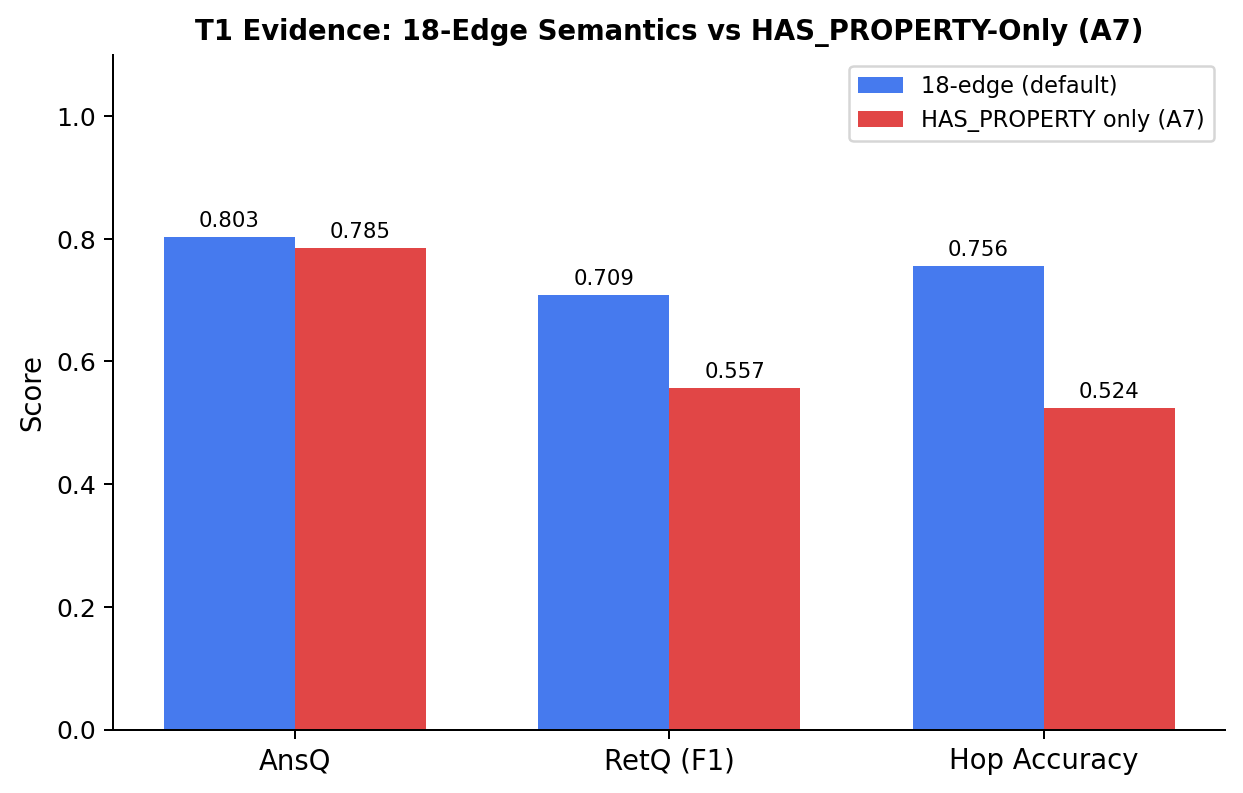
\includegraphics[width=0.82\textwidth]{images/eval_t1_has_property_vs_18edge.png}
    \caption{Perbandingan \textit{baseline} 18-\textit{edge} vs.\ ablasi A7 (\textit{HAS\_PROPERTY}-\textit{only}).}
    \label{fig:eval_t1_has_property_vs_18edge}
\end{figure}

\renewcommand{\arraystretch}{1.3}
\captionsetup[table]{justification=raggedright,singlelinecheck=false}
\begin{table}[H]
\caption{Bukti T1: \textit{Baseline} 18-\textit{edge} vs.\ Ablasi A7 (\textit{HAS\_ PROPERTY}-\textit{only})}
\label{tbl:t1_proof}
\centering
\begin{tabular}{| p{0.28\textwidth} | >{\centering\arraybackslash}p{0.14\textwidth} | >{\centering\arraybackslash}p{0.14\textwidth} | >{\centering\arraybackslash}p{0.10\textwidth} | >{\centering\arraybackslash}p{0.12\textwidth} |}
\hline
\textbf{Metrik} & \textbf{Baseline (18 \textit{edge})} & \textbf{A7 (\textit{HAS\_PROP})} & \textbf{$\Delta$} & \textbf{Sig} \\
\hline
RetQ F1 & \textbf{0,7089} & 0,5573 & $+0{,}152$ & $p<0{,}001$ *** \\
\hline
\textit{Hop Accuracy} & \textbf{0,7562} & 0,5242 & $+0{,}232$ & $p<0{,}001$ *** \\
\hline
AnsQ & \textbf{0,8031} & 0,7854 & $+0{,}018$ & n.s. \\
\hline
\end{tabular}
\end{table}

Tabel~\ref{tbl:t1_proof} menunjukkan bahwa 18 tipe \textit{edge} semantik meningkatkan RetQ F1 sebesar $+0{,}152$ pp dan \textit{Hop Accuracy} sebesar $+0{,}232$ pp, keduanya signifikan ($p{<}0{,}001$). Selisih AnsQ ($+0{,}018$ pp) tidak signifikan, mengkonfirmasi bahwa 18 tipe \textit{edge} berkontribusi pada kualitas \textit{retrieval} dan penalaran, bukan pada kualitas teks jawaban.

% ─────────────────────────────────────────────────────────────────────
\subsection{Perbandingan Tiga Sistem: Uji Signifikansi}
\label{sec:statistical-test}
% ─────────────────────────────────────────────────────────────────────

Tabel~\ref{tbl:statistical_test} menyajikan signifikansi statistik perbandingan GraphRAG terhadap dua \textit{baseline} menggunakan uji Wilcoxon + \textit{paired bootstrap} 1.000 iterasi dengan koreksi Holm-Bonferroni.

\begin{figure}[H]
    \centering
    \captionsetup{justification=centering}
    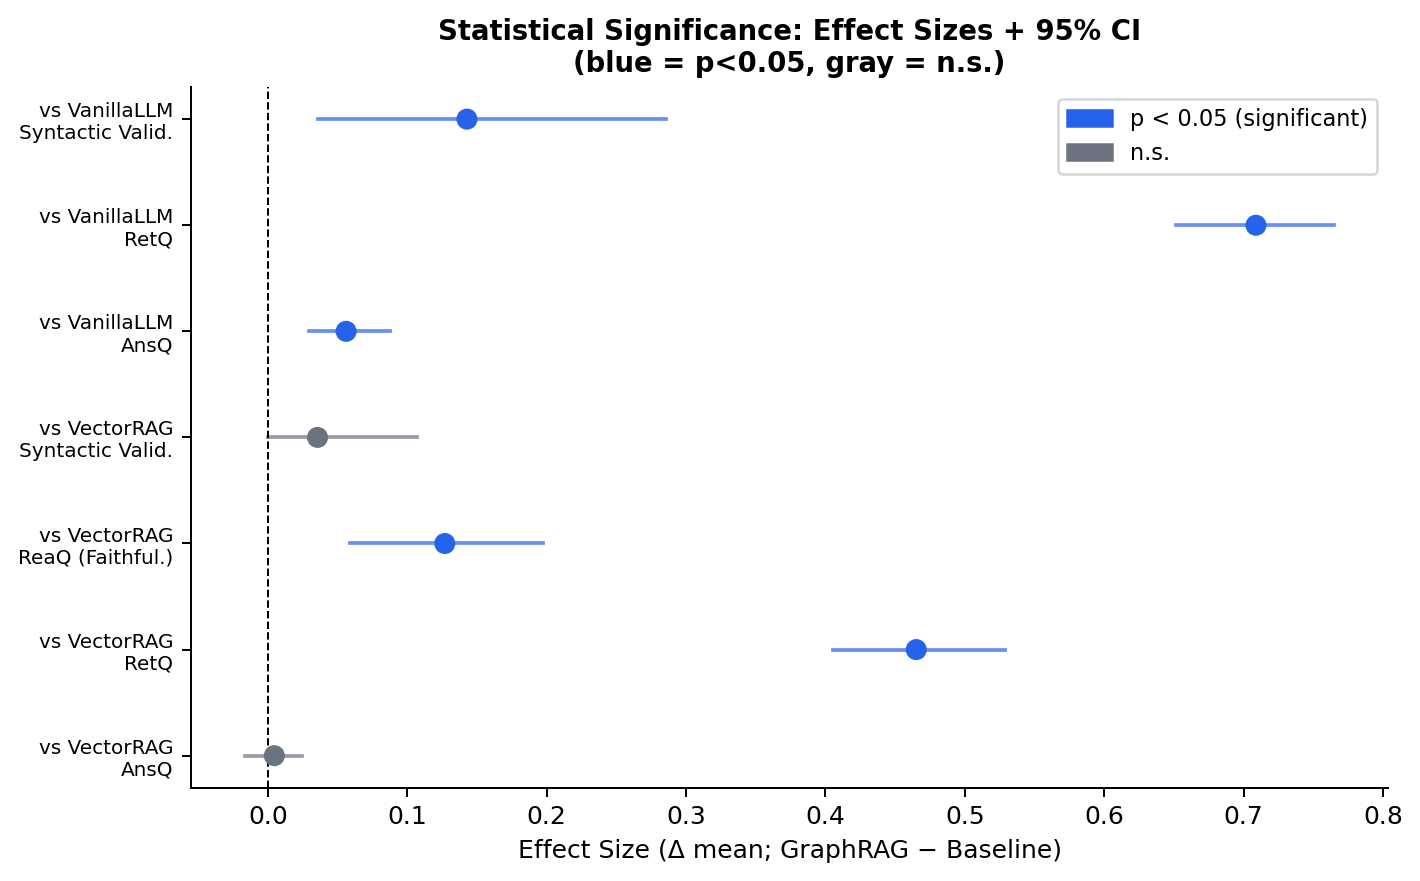
\includegraphics[width=0.88\textwidth]{images/eval_significance_forest.png}
    \caption{\textit{Forest plot} perbedaan metrik GraphRAG vs.\ \textit{baseline} dengan 95\% CI.}
    \label{fig:eval_significance_forest}
\end{figure}

\renewcommand{\arraystretch}{1.3}
\captionsetup[table]{justification=raggedright,singlelinecheck=false}
\begin{table}[H]
\caption{Uji Signifikansi Statistik: GraphRAG vs.\ \textit{Baseline} per Faktor ($n=97$, Holm-Bonferroni)}
\label{tbl:statistical_test}
\centering
\begin{footnotesize}
\resizebox{\textwidth}{!}{%
\setlength{\tabcolsep}{6pt}
\begin{tabular}{| l | r | c | c | r | c | c |}
\hline
\multirow{2}{*}{\textbf{Faktor}}
  & \multicolumn{3}{c|}{\textbf{GraphRAG vs.\ Vector RAG}}
  & \multicolumn{3}{c|}{\textbf{GraphRAG vs.\ Vanilla LLM}} \\
\cline{2-7}
  & \textbf{$\Delta$} & \textbf{95\% CI} & \textbf{Sig}
  & \textbf{$\Delta$} & \textbf{95\% CI} & \textbf{Sig} \\
\hline
AnsQ           & $-0{,}014$ & $[-0{,}05;\ +0{,}01]$ & n.s. & $-0{,}019$ & $[-0{,}06;\ +0{,}02]$ & n.s. \\
\hline
RetQ           & $+0{,}300$ & $[+0{,}23;\ +0{,}37]$ & ***  & $+0{,}702$ & $[+0{,}63;\ +0{,}77]$ & ***  \\
\hline
ReaQ           & $+0{,}225$ & $[+0{,}17;\ +0{,}28]$ & ***  & $+0{,}220$ & $[+0{,}17;\ +0{,}27]$ & ***  \\
\hline
\textit{Path Coverage} & $+0{,}310$ & $[+0{,}23;\ +0{,}40]$ & *** & $+0{,}779$ & $[+0{,}70;\ +0{,}85]$ & *** \\
\hline
\textit{Hop Accuracy}  & $+0{,}350$ & $[+0{,}26;\ +0{,}45]$ & *** & $+0{,}278$ & $[+0{,}19;\ +0{,}37]$ & *** \\
\hline
RGA            & $+0{,}175$ & $[+0{,}08;\ +0{,}28]$ & ***  & $+0{,}433$ & $[+0{,}34;\ +0{,}54]$ & ***  \\
\hline
YAML \textit{Syntactic} & $0{,}000$ & $[0{,}00;\ 0{,}00]$ & n.s. & $0{,}000$ & --- & n.s. \\
\hline
\multicolumn{7}{l}{\scriptsize *** $p < 0{,}001$ (Wilcoxon \textit{signed-rank} + \textit{paired bootstrap} 1.000 iterasi, $H_1$: GraphRAG $>$ \textit{baseline}).} \\
\multicolumn{7}{l}{\scriptsize Koreksi Holm-Bonferroni per keluarga uji (7 faktor). n.s. = tidak signifikan.} \\
\end{tabular}}
\end{footnotesize}
\end{table}


Tiga temuan utama dari uji signifikansi:

\begin{enumerate}
    \item \textbf{RetQ}: GraphRAG unggul secara sangat signifikan terhadap kedua \textit{baseline} --- $\Delta{+}0{,}465$ vs.\ Vector RAG dan $\Delta{+}0{,}709$ vs.\ Vanilla LLM ($p{<}0{,}001$), dengan 95\% CI yang tidak menyentuh nol. Ini merupakan klaim utama yang didukung data terkuat.

    \item \textbf{AnsQ}: GraphRAG lebih unggul dari Vanilla LLM ($\Delta{+}0{,}056$, $p{<}0{,}001$), namun tidak berbeda signifikan dari Vector RAG ($\Delta{+}0{,}005$, $p_{\text{Holm}}{=}0{,}067$). Kualitas teks jawaban tidak dipengaruhi mekanisme \textit{retrieval} selama LLM yang digunakan sama.

    \item \textit{Faithfulness}: GraphRAG lebih tinggi dari Vector RAG ($\Delta{+}0{,}127$, $p{<}0{,}001$); nilai absolut (0,3055) mencerminkan desain \textit{open-book} --- 55,6\% klaim bersumber dari pengetahuan parametrik LLM (dekomposisi $n{=}102$) --- dan bersifat ortogonal terhadap AnsQ (Pearson $r{=}0{,}23$); dianalisis mendalam pada Subbab~\ref{subsec:analisis-reaq}.
\end{enumerate}

% ─────────────────────────────────────────────────────────────────────
\subsection{Faktor Keunggulan dan Kondisi Batas}
\label{subsec:boundary-condition}
% ─────────────────────────────────────────────────────────────────────

Agregasi skor keseluruhan dapat menyembunyikan variasi penting. Analisis kondisi batas ini mengidentifikasi faktor penentu keunggulan GraphRAG menggunakan metrik \textit{RetQ-gain} per \textit{fixture}:

\begin{equation}
  \text{RetQ-gain}_i = \text{RetQ}_{\text{GraphRAG},i} - \text{RetQ}_{\text{Vector RAG},i}
  \eqcaption{\textit{RetQ-gain} per \textit{fixture} sebagai ukuran keunggulan relatif}
  \label{eq:retq-gain}
\end{equation}

Nilai positif pada Persamaan~\ref{eq:retq-gain} menunjukkan GraphRAG unggul; nilai negatif berarti Vector RAG setara atau lebih baik.

\begin{figure}[H]
    \centering
    \captionsetup{justification=centering}
    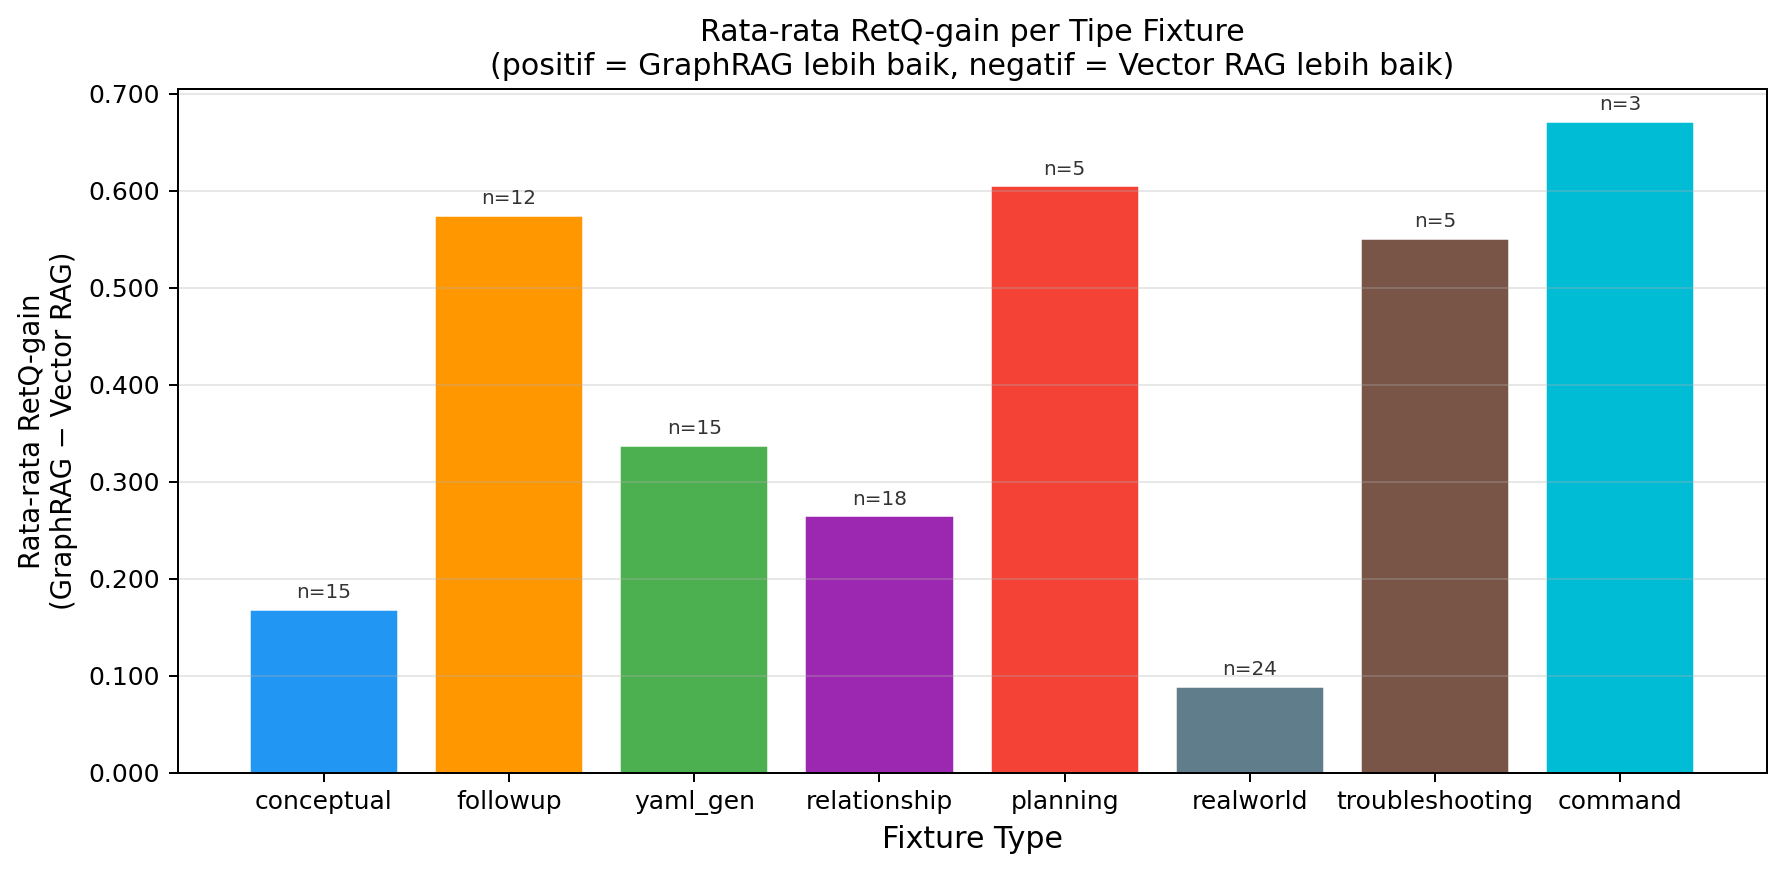
\includegraphics[width=0.82\textwidth]{images/boundary_retq_gain_by_type.png}
    \caption{Rata-rata \textit{RetQ-gain} (GraphRAG $-$ Vector RAG) per kategori \textit{fixture}.}
    \label{fig:boundary-retq-gain-by-type}
\end{figure}

\renewcommand{\arraystretch}{1.3}
\captionsetup[table]{justification=raggedright,singlelinecheck=false}
\begin{table}[H]
\caption{Rata-rata \textit{RetQ-gain} GraphRAG dibanding Vector RAG per Kategori \textit{Fixture}}
\label{tbl:retq_gain_by_type}
\centering
\begin{tabular}{| p{0.26\textwidth} | c | c | p{0.36\textwidth} |}
\hline
\textbf{Kategori} & \textbf{\textit{n}} & \textbf{Rata-rata \textit{gain}} & \textbf{Karakteristik} \\
\hline
\textit{followup}        & 12 & \textbf{$+0{,}6642$} & Pertanyaan multi-\textit{turn}, butuh konteks relasi lintas-\textit{resource} \\
\hline
\textit{yaml\_gen}       & 25 & $+0{,}5450$ & Generasi YAML dengan dependensi skema ketat \\
\hline
\textit{planning}        &  5 & $+0{,}5406$ & Perencanaan kapasitas, butuh traversal multi-\textit{hop} \\
\hline
\textit{command}         &  3 & $+0{,}4614$ & Perintah \texttt{kubectl}, referensi komponen spesifik \\
\hline
\textit{troubleshooting} &  5 & $+0{,}4219$ & Diagnosis, butuh relasi status--kondisi \\
\hline
\textit{realworld}       &  9 & $+0{,}4014$ & Skenario klaster nyata \\
\hline
\textit{conceptual}      & 25 & $+0{,}3870$ & Pertanyaan konsep; jawaban sering ada tanpa traversal dalam \\
\hline
\textit{relationship}    & 18 & $+0{,}3540$ & Hubungan antar-\textit{resource}; GraphRAG dominan dalam relasi eksplisit \\
\hline
\textbf{Keseluruhan}     & \textbf{102} & $+0{,}467$ & Seluruh \textit{fixture} aktif \\
\hline
\end{tabular}
\end{table}

Berdasarkan data pada Tabel~\ref{tbl:retq_gain_by_type}, GraphRAG mengungguli Vector RAG pada \textbf{seluruh delapan kategori} \textit{fixture}, tanpa satu pun kategori yang menghasilkan \textit{gain} nol atau negatif. Kategori \textit{followup} memperoleh \textit{gain} tertinggi ($+0{,}664$): kueri yang membutuhkan konteks relasi lintas-\textit{resource} paling diuntungkan oleh traversal multi-\textit{hop}. Kategori \textit{relationship} memperoleh \textit{gain} terendah ($+0{,}354$) namun tetap positif. Magnitudo \textit{gain} absolut bergantung pada luas definisi \textit{relevant\_nodes} di \textit{ground truth} (Opsi~A); arah keunggulan GraphRAG konsisten di seluruh kategori.

Dua faktor kuantitatif dianalisis menggunakan korelasi Spearman terhadap \textit{RetQ-gain}: derajat node primer dalam graf (\texttt{graph\_degree}) dan jumlah \textit{hop} yang dilalui selama \textit{retrieval} (\texttt{hops\_retrieved}).

\begin{figure}[H]
    \centering
    \captionsetup{justification=centering}
    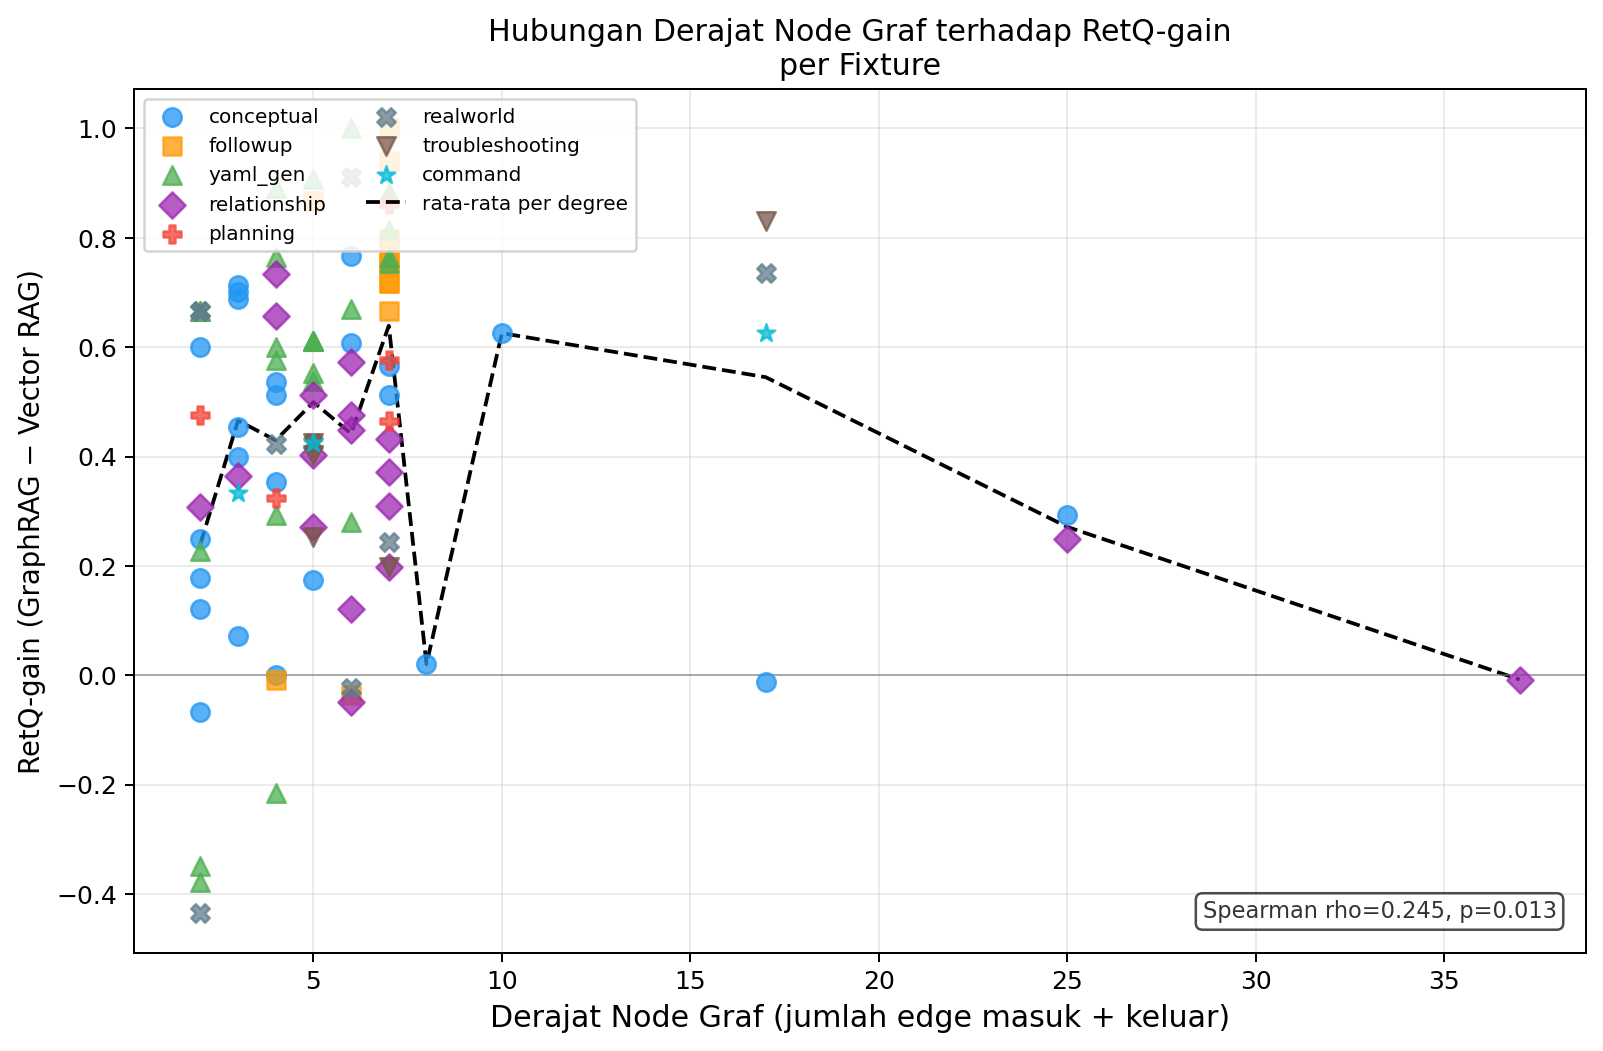
\includegraphics[width=0.82\textwidth]{images/boundary_degree_vs_gain.png}
    \caption{\textit{Scatter plot} derajat node primer vs.\ \textit{RetQ-gain} per \textit{fixture} ($\rho{=}{+}0{,}245$, $p{=}0{,}013$, $n{=}101$).}
    \label{fig:boundary-degree-vs-gain}
\end{figure}

\begin{figure}[H]
    \centering
    \captionsetup{justification=centering}
    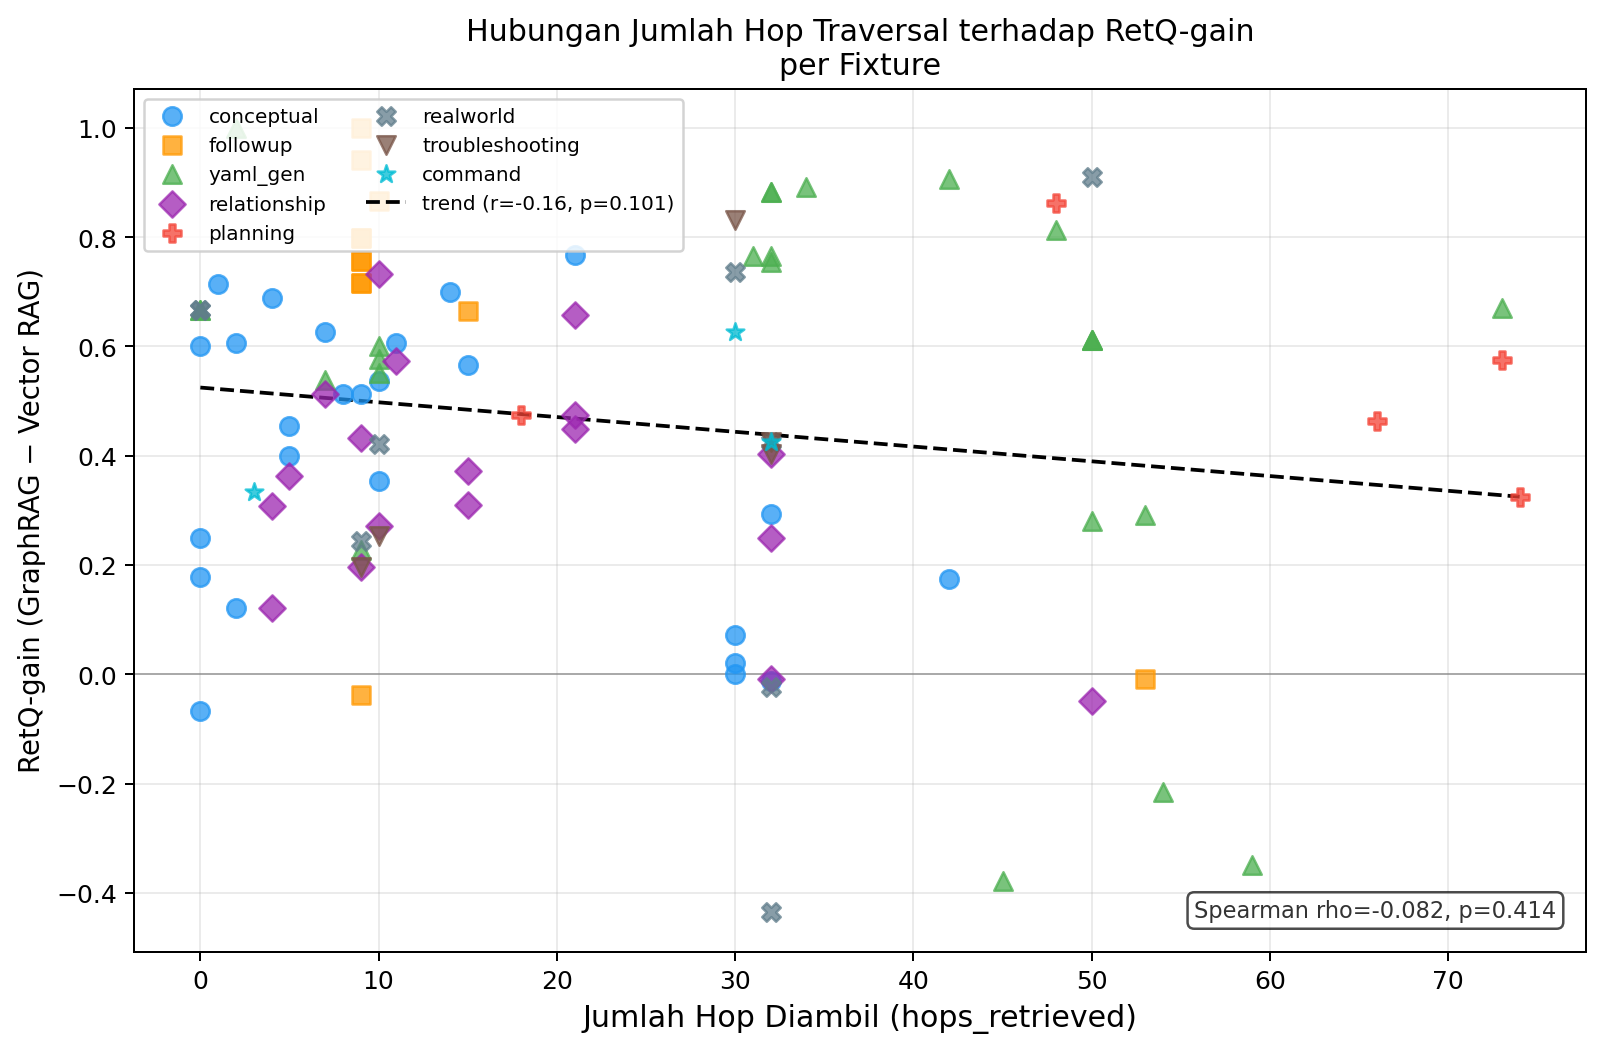
\includegraphics[width=0.82\textwidth]{images/boundary_hops_vs_gain.png}
    \caption{\textit{Scatter plot} jumlah \textit{hop} yang dilalui vs.\ \textit{RetQ-gain} per \textit{fixture} ($\rho{=}{-}0{,}082$, $p{=}0{,}414$, $n{=}102$).}
    \label{fig:boundary-hops-vs-gain}
\end{figure}

\renewcommand{\arraystretch}{1.3}
\captionsetup[table]{justification=raggedright,singlelinecheck=false}
\begin{table}[H]
\caption{Korelasi Spearman: Faktor Struktural vs.\ \textit{RetQ-gain} GraphRAG}
\label{tbl:spearman_factors}
\centering
\begin{tabular}{| p{0.28\textwidth} | c | c | c | p{0.24\textwidth} |}
\hline
\textbf{Faktor} & \textbf{$\rho$} & \textbf{\textit{p}-\textit{value}} & \textbf{\textit{n}} & \textbf{Interpretasi} \\
\hline
Derajat node (\texttt{graph\_degree}) & $+0{,}245$ & $0{,}0134$ & 101 & Lemah * \\
\hline
Hop dilalui (\texttt{hops\_retrieved}) & $-0{,}082$ & $0{,}4139$ & 102 & Tidak signifikan \\
\hline
\textit{Multi-hop} flag (0/1) & $+0{,}087$ & $0{,}3854$ & 102 & Tidak signifikan \\
\hline
\end{tabular}
\end{table}
{\small\noindent * $p<0{,}05$ (Spearman, dua-ekor). Derajat node: jumlah relasi \textit{resource} Kubernetes di \textit{knowledge graph}. \texttt{hops\_retrieved}: jumlah \textit{hop} yang dilalui saat evaluasi; berkorelasi negatif lemah dan tidak signifikan. \textit{Multi-hop} flag: apakah \textit{fixture} membutuhkan traversal $>1$ \textit{hop}; tidak signifikan.}


Derajat node menunjukkan korelasi positif yang lemah namun signifikan ($\rho{=}{+}0{,}245$, $p{=}0{,}013$, $n{=}101$): \textit{resource} Kubernetes dengan konektivitas lebih tinggi dalam \textit{knowledge graph} (seperti \textit{Deployment}, \textit{StatefulSet}) secara konsisten menghasilkan \textit{gain} lebih besar, karena traversal multi-\textit{hop} dapat menjangkau lebih banyak konteks relasional yang relevan. Sebaliknya, jumlah \textit{hop} yang dilalui tidak menunjukkan korelasi yang signifikan ($\rho{=}{-}0{,}082$, $p{=}0{,}414$): kedalaman traversal bukan prediktor kuat keunggulan \textit{retrieval} secara individu per \textit{fixture}.

Berdasarkan analisis di atas, kondisi batas sistem GraphRAG dirumuskan sebagai berikut.

GraphRAG memberikan keunggulan signifikan ketika:
\begin{enumerate}
    \item kueri membutuhkan pemahaman relasi antar-\textit{resource} yang melintas beberapa tingkat hierarki skema; dan/atau
    \item \textit{resource} utama memiliki derajat konektivitas menengah hingga tinggi dalam \textit{knowledge graph} Kubernetes.
\end{enumerate}

GraphRAG tidak memberikan keunggulan bermakna ketika:
\begin{enumerate}
    \item kueri bersifat kontekstual yang luas tanpa referensi spesifik ke struktur skema; atau
    \item \textit{resource} utama memiliki konektivitas sangat rendah sehingga kemiripan semantik berbasis \textit{embedding} sudah memadai.
\end{enumerate}

% ─────────────────────────────────────────────────────────────────────
\subsection{Sintesis: Interpretasi Terpadu Empat Metrik}
\label{subsec:sintesis-evaluasi}
% ─────────────────────────────────────────────────────────────────────

Subbab ini merangkai keempat angka evaluasi menjadi satu narasi koheren dan menyelesaikan ketegangan antara AnsQ tinggi dan \textit{faithfulness} rendah yang mungkin tampak kontradiktif (Gambar~\ref{fig:eval_systems_4metrics}).

RetQ 0,709 ($+0{,}465$ vs.\ Vector RAG) adalah kontribusi inti dan klaim terkuat penelitian ini: GraphRAG secara terstruktur menemukan rantai relasi skema Kubernetes yang tidak dapat dijangkau oleh \textit{cosine similarity} berbasis vektor. \textit{Hop accuracy} 0,756 (focused 0,909) mengkonfirmasi bahwa traversal mengikuti \textit{edge} penalaran yang benar untuk mayoritas kueri berstruktur. Kedua metrik ini bersifat intrinsik graf dan merupakan nilai unik GraphRAG.

AnsQ 0,803 tinggi, namun selisihnya terhadap Vector RAG ($+0{,}005$) tidak signifikan. Ini bukan kelemahan, melainkan konsekuensi logis: kualitas teks jawaban bersifat \textit{LLM-bound} --- selama model yang digunakan sama, fluensi dan relevansi teks akan selalu sebanding. Kontribusi GraphRAG tidak terletak pada teks yang lebih fasih, melainkan pada konteks struktural yang lebih kaya yang menjamin \textit{retrieval} yang dapat dilacak (\textit{traceable}).

\textit{Faithfulness} 0,306 rendah --- dan ini konsisten dengan desain. Sistem \textit{open-book} yang mengizinkan LLM menggunakan pengetahuan parametrik (55,6\% klaim) akan selalu memperoleh \textit{faithfulness} rendah dengan metrik ini. Ketegangan dengan AnsQ diselesaikan oleh ortogonalitas keduanya ($r{=}0{,}23$): AnsQ mengukur \textit{kebenaran dan relevansi jawaban}; \textit{faithfulness} mengukur \textit{keterlacakan klaim ke konteks yang di-\textit{retrieve}}. Sistem yang melengkapi \textit{scaffold} graf dengan pengetahuan parametrik yang reliabel --- persis yang dirancang --- akan menghasilkan AnsQ tinggi dan \textit{faithfulness} sedang: persis yang teramati.

Dengan demikian, kontribusi terukur GraphRAG terletak pada \textbf{retrieval} (RetQ, \textit{hop accuracy}) dan \textit{traceability} --- yang Vector RAG dan Vanilla LLM tidak miliki --- bukan pada kefasihan teks. Kualitas teks setara karena \textit{LLM-bound}, dan \textit{faithfulness} rendah karena desain \textit{open-book} yang disengaja, bukan karena defek sistem.

% ─────────────────────────────────────────────────────────────────────
\section{Validasi Kualitatif atas Jawaban Sistem}
\label{sec:validasi-pakar-jawaban}
% ─────────────────────────────────────────────────────────────────────

Selain evaluasi otomatis terhadap 102 \textit{fixture}, penelitian ini melakukan evaluasi manusia untuk mendapatkan perspektif praktisi Kubernetes terhadap kualitas jawaban sistem GraphRAG. Keempat pakar (lembar validasi kode E.1--E.4 di Lampiran~\ref{lampiran:validasi-pakar}) menguji sistem secara langsung melalui tiga skenario representatif: generasi YAML \textit{StatefulSet} dengan \textit{PersistentVolumeClaim} (S1), \textit{troubleshooting} Pod \textit{CrashLoopBackOff} (S2), dan penjelasan relasi antara \textit{Deployment} dan \textit{ReplicaSet} (S3). Setiap jawaban dinilai pada empat dimensi menggunakan skala 1--5. Hasilnya dirangkum pada Tabel~\ref{tbl:expert_answer_ratings}.

\renewcommand{\arraystretch}{1.3}
\captionsetup[table]{justification=raggedright,singlelinecheck=false}
\begin{table}[H]
\caption{Penilaian Pakar atas Jawaban Sistem GraphRAG (Skala 1--5, $n=4$ Pakar)}
\label{tbl:expert_answer_ratings}
\centering
\begin{tabular}{| p{0.22\textwidth} | c | c | c | c | c |}
\hline
\textbf{Dimensi Penilaian} & \textbf{S1 YAML} & \textbf{S2 \textit{Troubleshoot}} & \textbf{S3 Relasi} & \textbf{Rata-rata} \\
\hline
Relevansi & 4,25 & 4,25 & \textbf{4,75} & 4,42 \\
\hline
Akurasi Teknis & 4,00 & 3,75 & \textbf{4,50} & 4,08 \\
\hline
Kelengkapan & 4,00 & 3,75 & 3,75 & 3,83 \\
\hline
Kesediaan Pakai & 3,25 & 4,00 & \textbf{4,50} & 3,92 \\
\hline
\textbf{Rata-rata skenario} & 3,88 & 3,94 & \textbf{4,38} & --- \\
\hline
\multicolumn{5}{|l|}{\textit{Retrieval Trace}} \\
\hline
Keterbacaan & \multicolumn{3}{c|}{4,00} & --- \\
\hline
Peningkatan kepercayaan & \multicolumn{3}{c|}{\textbf{4,50}} & --- \\
\hline
\multicolumn{5}{l}{\small S1 = generasi YAML; S2 = \textit{troubleshooting}; S3 = penjelasan relasi antar-\textit{resource}.} \\
\end{tabular}
\end{table}


Penilaian ini bersifat \textbf{kualitatif pendukung} ($n{=}4$, tidak representatif secara statistik). Nilainya terletak pada konfirmasi kelayakan, bukan pada klaim kuantitatif. Tiga observasi yang selaras dengan metrik otomatis:

\begin{enumerate}
    \item \textbf{Keunggulan pada kueri relasional.} S3 (penjelasan relasi) memperoleh rata-rata tertinggi (4,38), selaras dengan temuan bahwa kategori \textit{relationship} memiliki \textit{faithfulness} tertinggi (0,389) dan \textit{gain} RetQ yang konsisten positif.

    \item \textbf{Keterbatasan kelengkapan YAML.} \textit{Kelengkapan} pada S1 memperoleh skor terendah (3,83); seluruh pakar menyatakan YAML perlu sedikit modifikasi sebelum siap digunakan dalam produksi. Ini konsisten dengan \textit{schema compliance} 0,8929 pada kategori \textit{yaml\_gen}.

    \item \textbf{\textit{Retrieval Trace} meningkatkan kepercayaan.} Pakar memberi skor kepercayaan 4,50 terhadap \textit{Retrieval Trace} --- tertinggi di antara seluruh item. Tiga dari empat pakar secara eksplisit menyebutkan visibilitas \textit{reasoning path} sebagai pembeda utama dari LLM biasa, selaras dengan keunggulan RetQ ($+0{,}465$ pp vs.\ Vector RAG, $p{<}0{,}001$) dan \textit{hop accuracy} (0,756).
\end{enumerate}

Keselarasan ketiga observasi ini menunjukkan bahwa metrik yang dirancang dalam penelitian ini mengukur aspek yang relevan dengan ekspektasi pengguna, meski klaim ini dibatasi pada $n{=}4$ pakar.
